\documentclass{praca1}
\usepackage[utf8]{inputenc}
\usepackage{tikz}
\usetikzlibrary{matrix, decorations.pathreplacing, calc, arrows}

%%------------------------------------------------------------------------------%

%------------------------------------------------------------------------------%

%\usepackage[dvips]{graphicx,color,rotating}
%\usepackage[utf8]{inputenc}
%\usepackage{t1enc}
%\usepackage{a4wide}
%\usepackage{amsfonts}
\usepackage{amsmath}
\usepackage{examplep}
\usepackage{xcolor}
\usepackage{mathtools}
\usepackage{cprotect}
\usepackage{algorithmicx}
\usepackage{algpseudocode}
\usepackage{algorithm}
%%\usepackage{enumitem}
%\usepackage{enumerate}
%\usepackage{verbatim}
%\usepackage[MeX]{polski}
%\usepackage[T1]{fontenc}
%\usepackage{geometry}
%\geometry{left=25mm,right=25mm,%
%bindingoffset=10mm, top=25mm, bottom=25mm}
%\usepackage{amssymb, latexsym}
%\usepackage{amsthm}
%\usepackage{palatino}
%\usepackage{array}
%\usepackage{pstricks}
%\usepackage{textcomp}
%\usepackage{hyperref}
%%paginy
%\usepackage{fancyhdr}
\DeclarePairedDelimiter{\norm}{\lVert}{\rVert}



\author{Natalia Potocka}
\title{Automatyczna kategoryzacja tematyczna tekstów przy użyciu metryk w przestrzeni ciągów znaków}
\supervisor{dr Marek Gągolewski}
\type{magisters}
\discipline{matematyka}
\monthyear{grudzień 2015}
\date{\today}
\album{237476}

\begin{document}
%\maketitle
%\tableofcontents
%
% %-----------Początek części zasadniczej-----------
%
%
%\chapter*{Wstęp}
%\addcontentsline{toc}{chapter}{Wstęp}
%COŚ tu będzie.

\chapter{Odległości na przestrzeni ciągów znaków}\label{metryki-na-przestrzeni-ciagow-znakow}
%\color{red}

\section{Podstawowe definicje}


\begin{definition}
Niech  $\Sigma = \{\sigma_1, \ldots, \sigma_k\}$ będzie skończonym uporządkowanym zbiorem o~liczności $|\Sigma|$, zwanym \emph{alfabetem}.~\emph{Napisem} nazywamy skończony ciąg znaków z~$\Sigma$.~Zbiór wszystkich napisów o~długości $n$~nad $\Sigma$~jest oznaczony przez $\Sigma^n$,~podczas gdy przez $\Sigma^* = \bigcup_{n=1}^{\infty}\Sigma^n$ rozumiemy zbiór wszystkich napisów utworzonych ze~znaków z~$\Sigma$~\cite{Boytsov2011:indexingmethods}.
\end{definition}

O~ile nie podano inaczej, używamy zmiennych $s,\ t,\ u,\ v,\ w,\ x,\ y$ jako oznaczenie napisów oraz $a,\ b,\ c$ do oznaczenia napisów jednoznakowych albo po~prostu \emph{znaków}. Pusty napis jest oznaczany przez $\varepsilon$. Przez $|s|$, dla każdego napisu $s \in \Sigma^*$, rozumiemy jego długość, czyli liczbę znaków w~napisie. Ciąg napisów i/lub znaków oznacza ich złączenie, np. $stu$ to napis powstały ze złączenia napisów $s, t$ oraz $u$, natomiast $abc$, to napis powstały ze złączenia znaków $a, b$ oraz $c$~\cite{Boytsov2011:indexingmethods}. Dla rozróżnienia napisów od~zmiennych reprezentujących napis, te~pierwsze oznaczamy pismem maszynowym, np.~\verb|napis|.

Poprzez $s_i$~rozumiemy $i$-ty znak z~napisu $s$,~dla każdego $i \in \{1,\ldots,|s|\}$. Podciąg kolejnych przylegających do~siebie znaków z~napisu nazywamy \emph{podnapisem}. Podnapisem napisu $s$,~który zaczyna się od~$i$-tego znaku, a~kończy na~$j$-tym znaku, oznaczamy przez $s_{i:j}$, tj. $s_{i:j} = s_is_{i+1}\ldots s_j$ dla $i \leq j$. Zakładamy również, że~jeśli $j < i$, to $s_{i:j} = \varepsilon$~\cite{Boytsov2011:indexingmethods,Loo2014:stringdist}.

\begin{definition}
Załóżmy, że~napis $s$~jest reprezentacją złączenia trzech, być może pustych, podnapisów $w$, $x$ i $y$, tj. $s = wxy$. Wówczas podnapis $w$ nazywamy \emph{przedrostkiem}, natomiast podnapis $y$ -- przyrostek~\cite{Boytsov2011:indexingmethods}.
\end{definition}

\begin{definition}
Podnapis złożony z kolejnych, przylegających do siebie, znaków napisu, o ustalonej długości $q$ jest nazywany \emph{$q$-gramem}. $q$-gramy o $q$ równym jeden, dwa lub trzy mają specjalne nazwy: \emph{unigram, bigram} i \emph{trigram}. Jeśli $q > |s|$, to $q$-gramy napisu $s$ są napisami pustymi~\cite{Boytsov2011:indexingmethods}.
\end{definition}

%\begin{definition}
%\emph{Napisem} nazywamy skończone złączenie symboli (znaków) ze~skończonego \emph{alfabetu}, oznaczonego przez $\Sigma$. Produkt kartezjański rzędu $q$, $\Sigma\times\ldots\times\Sigma$ oznaczamy przez $\Sigma^q$, natomiast zbiór wszystkich skończonych napisów, które można utworzyć ze~znaków z $\Sigma$ oznaczamy przez~$\Sigma^*$. \emph{Pusty napis}, oznaczany $\varepsilon$, również należy do~$\Sigma^*$. Napisy zwyczajowo będziemy oznaczać przez $s$,~$t$~oraz $u$,~a~ich \emph{długość}, czyli liczbę znaków w~napisie, przez $|s|$. Poprzez $s_i$ rozumiemy $i$-ty znak z napisu $s$, dla każdego $i \in \{1,\ldots,|s|\}$, natomiast podnapisy od znaku $i$-tego do znaku $j$-tego oznaczamy przez $s_{i:j}$. Zakładamy również, że jeśli $j<i$, to $s_{i:j} = \varepsilon$ \cite{Loo2014:stringdist}.
%\end{definition}


\begin{example}
Niech $\Sigma$ będzie alfabetem złożonym z~$26$ małych liter alfabetu łacińskiego oraz niech $s = \verb|ela|$. Wówczas mamy $|s| = 3$, $s \in \Sigma^3$ oraz $s \in \Sigma^*$. Co więcej, mamy $s_1 = \verb|e|$, $s_2 = \verb|l|$, $s_3 = \verb|a|$. Podnapis $1:2$ napisu $s$ to $s_{1:2} = \verb|el|$. W napisie tym mamy do czynienia jedynie z $q$-gramami o $q$ równym jeden, dwa oraz trzy, odpowiednio: $\verb|e|,\ \verb|l|,\ \verb|a|$; $\verb|el|,\ \verb|la|$ oraz $\verb|ela|$.
\end{example}


We wszystkich przykładach niniejszego rozdziału zakładamy, jeśli nie podano inaczej, że alfabet składa się z $32$ liter polskiego alfabetu oraz liter \verb|q|, \verb|v| i \verb|x|.

%[TU TRZEBA BARDZIEJ FORMALNIE! BOYTSOV STR. 4-7]Odległość $d(s,t)$ pomiędzy dwoma napisami $s$~i~$t$~to~minimalny koszt ciągu operacji potrzebnego do~przetransformowania $s$~w~$t$ (i~$\infty$, gdy taki ciąg nie istnieje). Koszt ciągu operacji jest sumą kosztów pojedynczych operacji. Przez operacje rozumiemy skończoną liczbę reguł w~formie $\delta(x, y) = a$, gdzie $x$~i~$y$ to różne podnapisy, a~$a$~to~nieujemna liczba rzeczywista. Kiedy już, przy pomocy operacji, podnapis $x$~zostanie przekształcony w~napis $y$,~żadne dalsze operacje nie mogą być wykonywane na~$y$~\cite{Navarro2001:guidedtour}.

%Zauważmy w~szczególności ostatnie ograniczenie, które nie pozwala wielokrotnie przekształcać tego samego podnapisu. DO POPRAWKI!!!: Gdyby pominąć to~założenie, każdy system przekształcający napisy spełniałby definicję i~stąd odległość między dwoma napisami nie byłaby, w~ogólności, możliwa do~policzenia~\cite{Navarro2001:guidedtour}.

%Jeśli dla każdej operacji $\delta(x,y)$, istnieje odpowiednia operacja $\delta(y,x)$ o~takim samym koszcie, to~odległość jest symetryczna (tj. $d(s,t) = d(t,s)$). Zauważmy również,~że:
%\begin{itemize}
%\item $d(s,t) \geq 0$ dla wszystkich napisów $s, t$,
%\item $d(s,s) = 0$,
%\item $d(s,u) \leq d(s,t) + d(t,u)$.
%\end{itemize}
%Stąd, jeśli odległość jest symetryczna, przestrzeń napisów tworzy przestrzeń metryczną~\cite{Navarro2001:guidedtour}.
%
%\begin{definition}
%\label{def:001}
%Funkcję $d$ nazywamy \emph{metryką} na~$\Sigma^*$, jeśli ma~poniższe własności:
%\begin{enumerate}
%\item \label{def:001a} $d(s,t) \geq 0$
%\item \label{def:001b} $d(s,t) = 0$ wtedy i tylko wtedy, gdy $s = t$
%\item \label{def:001c} $d(s,t) = d(t,s)$
%\item \label{def:001d} $d(s,u) \leq d(s,t) + d(t,u)$,
%\end{enumerate}
%gdzie $s$,~$t$,~$u$~są~napisami z~$\Sigma^*$.
%\end{definition}

%Z~powyższej definicji wynika, że~dla dowolnych $s,\ t \in \Sigma^*,\ d(s, t) \geq 0$.



\section{Odległości na przestrzeni ciągów znaków}

W niniejszym podrozdziale zajmiemy się odległościami na przestrzeni ciągów znaków, tj. funkcjami $d: \Sigma^* \times \Sigma^* \rightarrow [0, \infty)$. W literaturze można znaleźć wiele różnych funkcji tego typu, które różnią się genezą powstania, podejściem do problemu oraz zastosowaniami. W pracy zajmiemy się jednak odległościami, która można podzielić na~trzy garupy:
\begin{itemize}
\item oparte na~operacjach edycyjnych (\emph{edit operations}),
\item oparte na~$q$-gramach,
\item miary heurystyczne.
\end{itemize}

BLA BLA JAKIEŚ LANIE WODY O METRYKACH
Pierwszy rodzaj odległości jest najczęściej używany w algorytmach zajmujących się optymalnym dopasowaniem, dlatego też poświęcimy mu największą część niniejszego rozdziału. Odległości oparte na $q$-gramach ... (TUTAJ COŚ O NICH). Natomiast miary heurystyczne są rzadko stosowane, będąc zazwyczaj używane w konkretnych przypadkach. Miary te miały jednak swój wkład w historię optymalizacji [NIE!] napisów, zatem pokrótce opiszemy je pod koniec tego rozdziału.

\subsection{Odległości oparte na operacjach edycyjnych}

HISTORIA ODLEGLOSCI EDYCYJNYCH?

\textbf{Ścieżka edycyjna i bazowe operacje edycyjne.} \emph{Odległość edycyjna} $ED(s,t)$ między dwoma napisami $s$~i~$t$~to~minimalna liczba operacji edycyjnych potrzebna do~przetworzenia $s$~w~$t$ (i~$\infty$, gdy taki ciąg nie istnieje)~\cite{Navarro2001:guidedtour}. \emph{Ścisłą odległością edycyjną} nazywamy minimalną liczbę nienakładających się operacji edycyjnych, które pozwalają przekształcić jeden napis w drugi, i które nie przekształcają dwa razy tego samego podnapisu~\cite{Boytsov2011:indexingmethods}.

Napis może zostać przetworzony w drugi poprzez wykonanie na nim ciągu przekształceń jego podnapisów. Ten ciąg nazywany jest \emph{ścieżką edycyjną (śladem edycji?)}, podczas gdy przekształcenia są nazywane \emph{bazowymi operacjami edycyjnymi}. Bazowe operacje edycyjne, które polegają na przekształceniu napisu $s$ w napis $t$, są oznaczane przez $s \rightarrow t$. Zbiór wszystkich bazowych operacji edycyjnych oznaczamy przez~$\mathbb{B}$~\cite{Boytsov2011:indexingmethods}.


Bazowe operacje edycyjne są zazwyczaj ograniczone do:
\begin{itemize}
\item usunięcie znaku: $\verb|l| \rightarrow \varepsilon$, tj. usunięcie litery $\verb|l|$ , np. $\verb|ela| \rightarrow \verb|ea|$,
\item wstawienie znaku: $\varepsilon \rightarrow \verb|k|$, tj. wstawienie litery $\verb|k|$, np. $\verb|ela| \rightarrow \verb|elka|$,
\item zamiana znaku: $\verb|e| \rightarrow \verb|a|$, tj. zamiana litery $\verb|e|$ na $\verb|a|$, np. $\verb|ala| \rightarrow \verb|ela|$,
\item transpozycja: $\verb|el| \rightarrow \verb|le|$, tj. przestawienie dwóch przylegających liter $\verb|e|$ i $\verb|l|$, np. $\verb|ela| \rightarrow \verb|lea|$.
\end{itemize}

Często transpozycja znaków nie należy do zbioru operacji bazowych, jako że można ją zastąpić usunięciem i wstawieniem znaku. W niniejszej pracy jednak, operacja ta należy do zbioru operacji bazowych.

%Koszt wszystkich powyższych operacji zazwyczaj wynosi $1$. Dla wszystkich odległości, które dopuszczają więcej niż jedną operację edycyjną, może być znaczące nadanie wag poszczególnym operacjom, dając na przykład transpozycji mniejszy koszt niż operacji wstawienia znaku. Odległości, dla których takie wagi zostają nadane są zazwyczaj nazywane \emph{uogólnionymi} odległościami~\cite{Boytsov2011:indexingmethods}.

\begin{property}\label{wl:001}
Zakładamy, że $\mathbb{B}$ spełnia następujące własności~\cite{Boytsov2011:indexingmethods}:
\begin{itemize}
\item jeśli $s \rightarrow t \in \mathbb{B}$, to odwrotna operacja $t \rightarrow s$ również należy do $\mathbb{B}$;
\item $a \rightarrow a \in \mathbb{B}$ (operacja identycznościowa dla jednego znaku należy do $\mathbb{B}$);
\item zbiór $\mathbb{B}$ jest zupełny: dla dwóch dowolnych napisów $s$ i $t$, istnieje ślad edycji, który przekształca $s$ w $t$.
\end{itemize}
\end{property}

Zauważmy, że zbiór $\mathbb{B}$ nie musi być skończony.

\textbf{Odległość edycyjna.} Podobieństwo dwóch napisów może być wyrażone jako długość ścieżki edycyjnej, dzięki której jeden napis zostaje przekształcony w drugi:

\begin{definition}
Mając dany zbiór bazowych operacji edycyjnych, \emph{odległość edycyjna} $ED(s,t)$ jest równa długości najkrótszej ścieżki edycyjnej, która przekształca napis $s$ w napis $t$. Najkrótsza ścieżka, która przekształca napis $s$ w napis $t$ jest nazywana \emph{optymalną} ścieżką edycyjną~\cite{Boytsov2011:indexingmethods}. 
\end{definition}

\begin{example}
JAKIŚ PRZYKŁĄD SCIEZKI I OPTYMALNEJ SCIEZKI.
\end{example}

Przykładowe odległości edycyjne: Hamminga, najdłuższego wspólnego podnapisu (\emph{longest common substring}), Levenshteina, optymalnego dopasowania napisów (\emph{optimal string alignment}), Damareu-Levenshteina. Odległości te różnią się zbiorem bazowych operacji edycyjnych. Jeśli w zbiorze tym znajduje się tylko zamiana znaków, to mamy do czynienia z odległością Hamminga. Gdy zbiór bazowych operacji edycyjnych zawiera wstawienia i usunięcia znaków, to jest to odległość najdłuższego wspólnego podnapisu. Gdyby $\mathbb{B}$ powiększyć o zamianę znaków, to otrzymamy odległość Levenshteina. Dwie ostatnie odległości, tj. optymalnego dopasowania napisów oraz Damareu-Levenshteina, mają w zbiorze bazowych operacji edycyjnych usunięcie, wstawienie, zamianę oraz transpozycję znaków. Formalne definicje powyższych funkcji znajdują się w dalszej części niniejszego rozdziału.




Definicja odległości edycyjnej może być również interpretowana jako minimalny koszt, dzięki któremu przekształcamy jeden napis w drugi. Definicję można uogólnić na dwa sposoby. Po pierwsze, bazowe operacje edycyjne mogą mieć przydzielone koszty (wagi) $\delta(a \rightarrow b)$~\cite{Wagner1974:stringtostring}. Zazwyczaj koszt każdej operacji wynosi jeden, jednak można, na przykład, nadać transpozycji mniejszy koszt niż operacji wstawienia znaku. Dalej, można rozszerzyć funkcję kosztu $\delta$ na ścieżkę edycyjną $E = a_1 \rightarrow b_1, a_2 \rightarrow b_2, \ldots, a_{|E|} \rightarrow b_{|E|}$ przez $\delta(E) = \sum\limits_{i=1}^{|E|}\delta(a_i \rightarrow b_i)$~\cite{Boytsov2011:indexingmethods}. Odtąd przez odległość między napisem $s$ a napisem $t$ będziemy rozumieć minimalny ze wszystkich możliwych kosztów ścieżek przekształcających $s$ w $t$. Odległości zdefiniowane w ten sposób zazwyczaj są nazywane \emph{uogólnionymi} odległościami edycyjnymi.\\
Po drugie, zbiór operacji edycyjnych $\mathbb{B}$ może zostać rozszerzony o ważone zamiany (substytucje) (pod)napisów, zamiast operacji edycyjnych wykonywanych na pojedynczych znakach~\cite{Ukkonen1985:algorithmsforapprox}. Odległości zdefiniowane w ten sposób zazwyczaj są nazwyane \emph{rozszerzonymi} odległościami edycyjnymi. Przykładowo, $\mathbb{B}$ może zawierać operację $\verb|x| \rightarrow \verb|ks|$ o koszcie jednostkowym. Wówczas rozszerzona odległość pomiędzy napisami $\verb|xero|$ i $\verb|ksero|$ wynosi jeden, podczas gdy standardowa (zwykła, nierozszerzona) odległość wyniosłaby dwa~\cite{Boytsov2011:indexingmethods}.

\begin{definition}\label{def:002}
Mając dany zbiór bazowych operacji edycyjnych $\mathbb{B}$ oraz funkcję $\delta$,~która nadaje koszt wszystkim bazowym operacjom edycyjnym z~$\mathbb{B}$,~uogólniona odległość edycyjna między napisami $s$~i~$t$~jest zdefiniowana jako minimalny spośród kosztów wszystkich możliwych ścieżek edycyjnych, które przekształcają $s$~w~$t$~\cite{Boytsov2011:indexingmethods}.
\end{definition}

[KONFLIKT Z OSTATNIM ZDANIEM POPRZEDNIEGO AKAPITU - UOGOLNIONYMI ODL. ED.] Zazwyczaj koszt pojedynczej operacji z $\mathbb{B}$ jest równy jeden. Czasem jednak nadaje się poszczególnym operacjom różne koszty, dając np. transpozycji mniejszą wagę niż wstawieniu znaku. Gdy koszt wszystkich operacji jest równy jeden, to mówimy po prostu o odległości edycyjnej, natomiast gdy różne operacje mają różne wagi, to mówimy o \emph{uogólnionej} odległości edycyjnej.

\begin{property}\label{wl:002}
Zakładamy, że funkcja kosztu $\delta(s \rightarrow t)$ ma następujące własności~\cite{Boytsov2011:indexingmethods}:
\begin{itemize}
\item $\delta(s \rightarrow t) \in \mathbb{R}$ (koszt operacji jest liczbą rzeczywistą),
\item $\delta(s \rightarrow t) = \delta(t \rightarrow s)$ (symetria),
\item $\delta(s \rightarrow t) \geq 0,\ \delta(s \rightarrow s) = 0\text{ i } \delta(s \rightarrow t) = 0 \Rightarrow s = t$ (dodatnia określoność ??),
\item $\forall \gamma > 0$ zbiór bazowych operacji $\{s \rightarrow t \in \mathbb{B} | \delta(s \rightarrow t) < \gamma \}$ jest skończony (skończoność podzbioru bazowych operacji, których koszt jest ograniczony z góry).
\end{itemize}
\end{property}

Zauważmy, że ostatnia własność jest zawsze spełniona dla skończonego zbioru $\mathbb{B}$.

\begin{theorem}
Z własności \ref{wl:001} i \ref{wl:002} wynika, że:
\begin{itemize}
\item dla każdych dwóch napisów $s$ i $t$, istnieje ścieżka o minimalnym koszcie, tj. dobrze zdefiniowana odległość edycyjna z $s$ do $t$~\cite{Boytsov2011:indexingmethods},
\item ogólna odległość edycyjna z definicji \ref{def:002} jest metryką~\cite{Wagner1974:stringtostring}.
\end{itemize}
\end{theorem}

\begin{proof}
Żeby udowodnić, że $ED(s,t)$ jest metryką, musimy pokazać, że $ED(s,t)$ istnieje, 	jest dodatnio określona, symetryczna oraz subaddytywna (tj. spełnia nierówność trójkąta).

Z własności~\ref{wl:002} wynika, że funkcja kosztu jest nieujemna (JA TEGO NIW WIDZE) i że tylko identyczność ma koszt równy zero. Stąd, bez utraty ogólności, możemy rozważyć jedynie takie ścieżki edycyjne, które nie zawierają operacji identycznościowych. Zatem, jeśli $s=t$, to jedyna optymalna ścieżka (która nie zawiera operacji identycznościowych) jest pusta i ma zerowy koszt. Jeśli $s\neq t$, to z zupełności zbioru bazowych operacji edycyjnych wynika, że istnieje jedna lub więcej ścieżek edycyjnych, które przekształcają $s$ w $t$. Wszystkie te ścieżki składają się z operacji edycyjnych o ściśle dodatnim koszcie.

Niech $\gamma$ będzie kosztem ścieżki przekształcającej $s$ w $t$. Rozważmy zbiór $A$ ścieżek edycyjnych, które przekształcają $s$ w $t$ i których koszt jest ograniczony z góry przez $\gamma$. Zbiór $A$ jest niepusty i składa się z operacji edycyjnych o dodatnim koszcie mniejszym niż $\gamma$. Zbiór operacji bazowych, których koszt jest ograniczony z góry przez $\gamma$ jest skończony, co dowodzi, że zbiór $A$ jest również skończony. Ponieważ $A$ jest niepusty i skończony, to ścieżki edycyjne o mininalnym (dodatnim) koszcie istnieją i należą do $A$. Stąd, $ED(s,t) > 0$ dla $s\neq t$, tj. odległość edycyjna jest dodatnio określona.

Aby udowodnić symetrię odległości edycyjnej, rozważmy optymalną ścieżkę $E$, która przekształca $s$ w $t$, oraz odpowiadającą jej odwrotną ścieżkę $E_r$, która przekształca $t$ w $s$. Równość ich kosztów $\delta(E) = \delta(E_r)$ wynika z symetrii funkcji kosztu i symetrii zbioru operacji bazowych~$\mathbb{B}$. 

Aby pokazać subaddytywność, rozważmy optymalną ścieżkę $E_1$, która przekształca $s$ w $t$, optymalną ścieżkę $E_2$, która przekształca $t$ w $u$, oraz złożenie ścieżek $E_1E_2$, które przekształca $s$ w $u$. Z tego, że $\delta(E_1E_2) = \delta(E_1) + \delta(E_2) = ED(s,t)+ED(t,u)$ oraz $\delta(E_1E_2) \geq ED(s,u)$ (gdyż $E_1 E_2$ nie musi być optymalną ścieżka, przekształcającą $s$ w $u$) wynika, że $ED(s,t)+ED(t,u) \geq ED(s,u)$.
\end{proof}

Odległość edycyjna jest metryką, nawet gdy funkcja kosztu $\delta$ nie jest subaddytywna. Co więcej, ponieważ ciąg nakładających się operacji, które przekształcają $s$ w $t$, mogą mieć mniejszy koszt niż $\delta(s \rightarrow t)$, $\delta(s \rightarrow t)$ może być większe niż $ED(s,t)$. Rozważmy, na przykład, następujący alfabet: $\{\verb|a, b, c|\}$, gdzie symetria i brak subaddytywności funkcji $\delta$ jest zdefiniowana następująco:
\begin{align*}
\delta(\PVerb{a} \rightarrow \PVerb{c}) &= \delta(\PVerb{b} \rightarrow \PVerb{c}) = 1 \\
\delta(\PVerb{a} \rightarrow \varepsilon) &= \delta(\PVerb{b} \rightarrow \varepsilon) = \delta(\PVerb{c} \rightarrow \varepsilon) = 2 \\
\delta(\PVerb{a} \rightarrow \PVerb{b}) &= 3
\end{align*}

Można zobaczyć, że $3 = \delta(\verb|a| \rightarrow \verb|b|) > \delta(\verb|a| \rightarrow \verb|c|) + \delta(\verb|c| \rightarrow \verb|b|) = 2$. Stąd optymalna ścieżka edycyjna $(\verb|a| \rightarrow \verb|c|, \verb|c| \rightarrow \verb|b|)$ przekształca $\verb|a|$ w $\verb|b|$ z kosztem równym $2$.

\textbf{Ścisła odległość edycyjna.} Subaddytywność odległości edycyjnej pozwala używać metod właściwych przestrzeniom metrycznym. Niemniej jednak, problem minimalizacji zbioru nakładających się operacji edycyjnych, może być trudny. Aby zrównoważyć złożoność obliczeniową, zazwyczaj używana jest funkcja podobieństwa, zdefiniowana jako minimum kosztu \emph{ścisłej ścieżki edycyjnej}. Ta ostatnia nie zawiera nakładających się na siebie operacji edycyjnych i nie modyfikuje tego samego podnapisu więcej niż raz. Odpowiająca jej odległość edycyjna nazywana jest \emph{ścisłą odległością edycyjną}~\cite{Boytsov2011:indexingmethods}.

\begin{lemma}
Dowolna nieścisła odległość edycyjna ogranicza z dołu odpowiadającą jej ścisłą odległość edycyjną~\cite{Boytsov2011:indexingmethods}.
\end{lemma}

\begin{lemma}
\label{lem:001}
Ścisła odległość Levenshteina o jednostkowym koszcie operacji bazowych jest równa nieścisłej odległości Levenshteina o jednostkowym koszcie operacji bazowych~\cite{Boytsov2011:indexingmethods}.
\end{lemma}

Powyższe wynika natychmiast z obserwacji, że optymalna ścieżka edycyjna zawiera jednoznakowe usunięcia, wstawienia oraz zamiany, które nigdy nie modyfikują podnapisu więcej niż raz.

\begin{lemma}
Nieścisła odległość Damerau-Levenshteina oraz ścisła odległość Damerau-Levenshteina są różnymi funkcjami. Co więcej ścisła odległość Damerau-Levenshteina nie jest metryką, gdyż nie jest subaddytywna~\cite{Boytsov2011:indexingmethods}.
\end{lemma}

\begin{proof}
Ścisła odległość Damerau-Levenshteina traktuje transpozycję (tj. zamianę dwóch przylegających do siebie znaków) jako bazową operację edycyjną. Aby udowodnić lemat podamy przykłąd, w którym zakaz modyfikacji znaków już stransponowanych odróżnia odległość Damerau-Levenshteina od ścisłej odległości Damerau-Levenshteina~\cite{Boytsov2011:indexingmethods}.
\end{proof}

Rozważmy napisy \verb|ab|, \verb|ba| oraz \verb|acb|. Z jednej strony, najkrótsza nieścisła ścieżka edycyjna, która przekształca \verb|ba| w \verb|acb|, tj. $(\verb|ba| \rightarrow \verb|ab|, \varepsilon \rightarrow \verb|c|)$ zawiera dwie operacje: najpierws zamienia znaki \verb|a| i \verb|b|, a następnie wstawia \verb|c| pomiędzy nie. Zauważmy, że wstawienie przekształca już transformowany napis. Jednakowoż, jeśli kolejne przekształcenia tego samego podnapisu są wykluczone, to najkrótsza ścieżka edycyjna, która przekształca \verb|ba| w \verb|acb|, składa się z trzech operacji edycyjnych, np. $(\verb|ba| \rightarrow \varepsilon, \varepsilon \rightarrow \verb|c|, \varepsilon \rightarrow \verb|b|)$. Stąd, nieścisła odległość edycyjna jest równa dwa, podczas gdy ścisła odległość wynosi trzy~\cite{Boytsov2011:indexingmethods}. 

Ścisła odległość Damerau-Levenshteina nie spełnia nierówności trójkąta, gdyż
$$
\verb|ba|  \xrightarrow[1]{transp.\ b\ i \ a} \verb|ab| + \verb|ab| \xrightarrow[1]{wst. c} \verb|acb|,
$$
natomiast
$$
\verb|ba|  \xrightarrow[1]{us.\ b} \verb|a| \xrightarrow[1]{wst.\ c} \verb|ac| \xrightarrow[1]{wst.\ b} \verb|acb|,
$$
zatem
$$
2 = ED(\verb|ba|, \verb|ab|) + ED(\verb|ab|, \verb|acb|) \leq ED(\verb|ba|, \verb|acb|) = 3.
$$

Ponieważ ścisła i nieścisła odległość Damerau-Levenshteina są różnymi funkcjami, tę pierwszą nazywa się często \emph{odległością optymalnego dopasowania napisów}. Od tego momentu w niniejszej pracy ścisłą odległość Damerau-Levenshteina nazywamy odległością optymalnego dopasowania napisów, natomiast nieścisłą odległość Damerau-Levenshteina nazywamy odległością Damerau-Levenshteina~\cite{Loo2014:stringdist}.

\textbf{Optymalne dopasowanie.} % Problem optymalnego obliczenia odległości Damerau-Levenshteina został rozwiązany przez Lowrance'a i Wagnera~\cite{Wagner1975:extensionstring}. W dalszej części podajemy formalne definicje oraz przegląd klasycznych dynamicznych algorytmów wyliczających odległość Levenshteina.

Niech napisy $s$ i $t$ zostaną podzielone na tę samą liczbę, być może pustych, podnapisów: $s = s_1 s_2 \ldots s_l$ i $t = t_1 t_2 \ldots t_l$, takich, że $s_i \rightarrow t_i \in \mathbb{B}$. Co więcej, zakładamy, że $s_i$ i $t_j$ nie mogą być puste dla $i = j$. Mówimy, że ten podział definiuje \emph{dopasowanie} $A = (s_1 s_2\ldots s_l, t_1 t_2 \ldots t_l)$ pomiędzy napisami $s$ i $t$, w którym podnapis $s_i$ jest dopasowany do podnapisu $t_i$~\cite{Boytsov2011:indexingmethods}.

Dopasowanie reprezentuje ścisłą ścieżkę edycyjną $E = s_1 \rightarrow t_1, s_2 \rightarrow t_2, \ldots, s_l \rightarrow t_l$. Definiujemy \emph{koszt dopasowania} $A$ jako koszt odpowiadającej mu ścieżki edycyjnej i oznaczamy go przez $\delta(A)$:

\begin{equation}
\label{eq:003}
\delta(A) = \sum\limits_{i = 1}^{l} \delta(s_i \rightarrow t_i)
\end{equation}

\emph{Optymalne dopasowanie} to dopasowanie o najmniejszym koszcie~\cite{Boytsov2011:indexingmethods}.


\begin{example}
Przykład optymalnego dopasowania pomiędzy słowami \verb|foczka| i \verb|kozak| prezentuje rys.~\ref{rys:001}. Odpowiadająca mu ścieżka edycyjna składa się z zamiany $\verb|f| \rightarrow \verb|k|$, usunięcia $\verb|c| \rightarrow \varepsilon$ oraz transpozycji $\verb|ka| \rightarrow \verb|ak|$.
\end{example}

\begin{figure}[width=80pt]
\centering
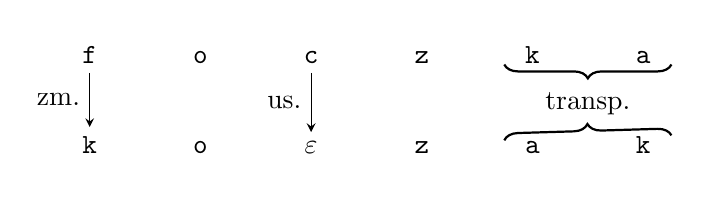
\begin{tikzpicture}
  \matrix (m) [matrix of math nodes,row sep=2em,column sep=2em,minimum width=2em]
  {
  	 \verb|f| & \verb|o| & \verb|c| & \verb|z| & \verb|k| & \verb|a| \\
     \verb|k| & \verb|o| & \varepsilon & \verb|z| & \verb|a| & \verb|k| \\};
  \path[-stealth]
    (m-1-1) edge node [left] {zm.} (m-2-1)
           
    (m-1-3) edge node [left] {us.} (m-2-3)
    
    ;
    
    \draw[decorate,decoration={brace,amplitude=5pt,mirror},transform canvas={yshift=0.3em},thick] (m-1-5.south west) -- node[yshift=-1.4em] { transp. } (m-1-6.south east);
     \draw[decorate,decoration={brace,amplitude=5pt},transform canvas={yshift=-0.3em},thick] (m-2-5.north west) -- node[yshift=-1.4em] { } (m-2-6.north east);
\end{tikzpicture}
\cprotect\caption{Przykład optymalnego dopasowania między napisami \verb|foczka| i \verb|kozak|.}\label{rys:001}
\end{figure}

Warto zauważyć, że istnieje różnowartościowe (1-1) mapowanie między zbiorem ścisłych ścieżek edycyjnych i zbiorem [optymalnych?] dopasowań: każda ścisła ścieżka edycyjna o minimalnym koszcie reprezentuje dopasowanie o najmniejszym koszcie i odwrotnie. Stąd można zastąpić problem znalezienia optymalnej ścisłej odległości edycyjnej poprzez problem znalezienia optymalnego dopasowania, co też zastosujemy dalej~\cite{Boytsov2011:indexingmethods}.

\textbf{Obliczanie odległości edycyjnej.} Główną zasadą dynamicznego algorytmu, liczącego koszt optymalnego dopasowania, jest wyrażenie kosztu dopasowania pomiędzy napisami $s$ i $t$, używając kosztu dopasowania ich przedrostków. Rozważmy prefiks $s_{1:i}$ o długości $i$ i przedrostek $t_{1:j}$ o długości $j$, odpowiednio napisów $s$ i $t$. Załóżmy, że $A = (s_1 s_2\ldots s_l, t_1 t_2 \ldots t_l)$ jest optymalnym dopasowaniem między $s_{1:i}$ i $t_{1:j}$, którego koszt oznaczamy przez $C_{i,j}$~\cite{Boytsov2011:indexingmethods}.

Używając równania \ref{eq:003} oraz definicji optymalnego dopasowania, łatwo pokazać, że $C_{i,j}$ może zostać policzone przy użyciu następującej ogólnej rekurencji~\cite{Ukkonen1985:algorithmsforapprox}:


\begin{align}
\begin{split}
\label{eq:004}
C_{0,0} &= 0 \\
C_{i,j} &= \min\{\delta(s_{i^\prime:i}\rightarrow t_{j^\prime:j}) + C_{i^\prime-1, j^\prime-1} | s_{i^\prime:i}\rightarrow t_{j^\prime:j} \in \mathbb{B}\}.
\end{split}
\end{align}

%Rekurencja \ref{eq:004} jest przykładem dynamicznego programowania. Zbiór liczb $\{C_{i,j}\}$ o liczności $(|s|+1)\cdot (|t|+1)$ jest zazwyczaj nazywany \emph{macierzą dynamicznego programowania} (lub w skrócie macierzą DP). Co więcej, 
Można zauważyć, że:
\begin{itemize}
\item koszt dopasowania napisów $s$ i $t$ jest równy $C_{|s|, |t|}$;
\item wszystkie optymalne dopasowania mogą zostać wyznaczone przez odwracanie rekurencji \ref{eq:004} (przechodzenie od tyłu), tj. obliczanie najpierw $C_{0,0}$, następnie $C_{1,1}$ itd.
\end{itemize}




Rozważmy teraz odległość Hamminga, gdzie $s_{i^\prime:i}\rightarrow t_{j^\prime:j}$ to zamiany znaków o koszcie równym jeden. Stąd,
\begin{equation}
\label{eq:005}
\delta(s_{i^\prime:i}\rightarrow t_{j^\prime:j}) = [s_{i^\prime:i}\neq t_{j^\prime:j}]
\end{equation}

gdzie $[X]$ jest równe jeden, gdy warunek $X$ jest spełniony, zero w przeciwnym przypadku. Co więcej, w tym przypadku możliwa jest tylko jedna kombinacja $i^\prime$ oraz $j^\prime$, mianowicie $i^\prime = i$ oraz $j^\prime = j$. Dalej, odległość ta jest zdefiniowana jedynie dla $|s| = |t|$, zatem $C_{i,j}$ może być policzone jedynie dla $i = j$. Wówczas definicja odległości Hamminga nie jest rekurencyjna i można ją zapisać następująco:


\begin{definition}
\emph{Odległością Hamminga} nazywamy~\cite{Hamming1950:errordetecting}:
$$
d_{\mathrm{hamming}}(s, t) = \left\{
\begin{array}{l l}     
    \sum\limits_{i=1}^{|s|}\delta(s_i \rightarrow t_i) = \sum\limits_{i=1}^{|s|}[s_i\neq t_i], & \text{gdy } |s| = |t|,\\
    \infty, & \text{w przeciwnym przypadku},
\end{array}\right.
$$
%gdzie 
%$$
%\delta(s_i, t_i) = \left\{
%\begin{array}{l l}     
%    1, & \text{gdy } s_i = t_i,\\
%    0, & \text{w przeciwnym przypadku}.
%\end{array}\right.
%$$
\end{definition}

%Odległość Hamminga dopuszcza jedynie zamianę znaku, stąd jest zdefiniowana tylko dla napisów o~równej długości. 
%Łatwo zauważyć, że~odległość Hamminga spełnia definicję metryki. 
Odległość Hamminga zlicza liczbę indeksów (p. rys.~\ref{rys:002}), na~których dwa napisy mają różny znak. Odległość ta~przyjmuje wartości ze~zbioru $\{0,\ldots,|s|\}$, gdy $|s|=|t|$, natomiast jest równa nieskończoności, gdy napisy mają różne długości.

[PIĘKNY RYSUNEK]


\begin{figure}[width=80pt]
\centering
\begin{tikzpicture}
  \matrix (m) [matrix of math nodes,row sep=2em,column sep=2em,minimum width=2em]
  {
     \verb|k| & \verb|o| & \verb|z| & \verb|a| \\
     \verb|f| & \verb|o| & \verb|k| & \verb|a| \\[-1.75em]
      1 & 2 & 3 & 4 \\ };
  \path[-stealth]
    (m-1-1) edge node [left] {zm.} (m-2-1)
           
    (m-1-3) edge node [left] {zm.} (m-2-3)
    
    ;
    
\end{tikzpicture}
\cprotect\caption{Przykład dopasowania przy pomocy odległości Hamming między napisami \verb|koza| i \verb|foka|.}\label{rys:002}
\end{figure}

\begin{example}
Odległość Hamminga między słowami \verb|koza| i \verb|foka| wynosi $d_{\mathrm{hamming}}(\verb|koza|, \verb|foka|) = 2$, natomiast między słowami \verb|kozak| i \verb|foczka| wynosi ona $d_{\mathrm{hamming}}(\verb|kozak|, \verb|foczka|) = \infty$, gdyż $|\verb|kozak| | \neq | \verb|foczka| |$.
\end{example}




Rozważmy teraz odległość najdłuższego wspólnego podnapisu, gdzie $s_{i^\prime:i}\rightarrow t_{j^\prime:j}$ to wstawienia i usunięcia znaków o koszcie równym jeden. Wówczas istnieją dwie kombinacje $i^\prime$ oraz $j^\prime$ z ogólnej rekurencji \ref{eq:005}, odpowiadające usunięciu i wstawieniu, odpowiednio:
\begin{itemize}
\item $i^\prime = i - 1$ oraz $j^\prime = j$,
\item $i^\prime = i$ oraz $j^\prime = j - 1$.
\end{itemize}

Uwzględniając powyższe uproszczenia, możemy następująco przepisać ogólną postać rekurencji \ref{eq:004} dla odległości najdłuższego wspólnego podnapisu [NIE WIEM CZY TO JEST DOBRZE!!!!]:

\begin{equation*}
C_{i,j} = \min\left\{
\begin{array}{l l}     
    0, & \text{gdy } i = j = 0 \\
    C_{i-1, j} + 1, & \text{gdy } i > 0 \\
    C_{i, j-1} + 1, & \text{gdy } j > 0
\end{array}\right.
\end{equation*}


%\begin{definition}
%\emph{Odległością najdłuższego wspólnego podnapisu}~\cite{Needleman2008:generalmethod} na $\Sigma^*$ nazywamy:
%$$
%d_{\mathrm{lcs}}(s, t) = \left\{
%\begin{array}{l l}     
%    0, & \text{gdy } s = t = \varepsilon,\\
%    d_{\mathrm{lcs}}(s_{1:|s|-1}, t_{1:|t|-1}), & \text{gdy } s_{|s|} = t_{|t|}, \\
%    1+min\{d_{\mathrm{lcs}}(s_{1:|s|-1}, t), d_{\mathrm{lcs}}(s, t_{1:|t|-1})\}, & \text{w przeciwnym przypadku},
%\end{array}\right.
%$$
%\end{definition}

Odległość najdłuższego wspólnego podnapisu przyjmuje wartości ze zbioru $\{0, |s|+|t|\}$, przy czym maksimum jest osiągane, gdy $s$ i $t$ nie mają ani jednego wspólnego znaku. Odległość tę oznaczamy przez $d_{\mathrm{lcs}}$.
%Odległość ta zlicza liczbę usunięć i~wstawień, potrzebnych do~przetworzenia jednego napisu w~drugi. 

\begin{example}
Odległość najdłuższego wspólnego podnapisu między napisami \verb|kozak| i \verb|foczka| wynosi: $d_{lsc}(\verb|kozak|, \verb|foczka|) = 5$, bo~$\verb|kozak|\xrightarrow[1]{us.\ k} \verb|ozak| \xrightarrow[1]{us.\ a} \verb|ozk| \xrightarrow[1]{wst.\ f} \verb|fozk| \xrightarrow[1]{wst.\ c} \verb|foczk| \xrightarrow[1]{wst.\ a} \verb|foczka|$.
\end{example}

Powyższy przykład pokazuje, że~w~ogólności nie ma~unikalnej najkrótszej drogi transformacji jednego napisu w~drugi, gdyż można zamienić kolejność usuwania (lub wstawiania) znaków i~również uzyskać odległość równą~$5$. Można również usunąć z napisu znak \verb|k| zamiast \verb|a|, otrzymując taką samą odległość między napisami.

Jak sugeruje nazwa, odległość najdłuższego wspólnego podnapisu, ma~też inną interpretację. Poprzez wyrażenie \emph{najdłuższy wspólny podnapis} rozumiemy najdłuższy ciąg utworzony przez sparowanie znaków z~$s$~i~$t$~nie zmieniając ich porządku. Wówczas odległość ta~jest rozumiana jako liczba niesparowanych znaków z~obu napisów. W~powyższym przykładzie może to~być zwizualizowane następująco (rys.~\ref{rys:003}):
	
	

\begin{figure}[width=80pt]
\centering
\begin{tikzpicture}
  \matrix (m) [matrix of math nodes,row sep=2em,column sep=1em,minimum width=2em]
  {
  	 \verb|k| & \verb|o| & \verb|z| & \verb|a| & \verb|k|  \\
  	 \verb|f| & \verb|o| & \verb|c| & \verb|z| & \verb|k| & \verb|a| \\[2em]
  	 \verb|k| & \verb|o| & \verb|z| & \verb|a| & \verb|k|  \\
  	 \verb|f| & \verb|o| & \verb|c| & \verb|z| & \verb|k| & \verb|a| \\
     };
  \path[-stealth]
    (m-1-2) edge node [left] {} (m-2-2)
           
    (m-1-3) edge node [left] {} (m-2-4)
    
    (m-1-5) edge node [left] {} (m-2-5)
    
    
    (m-3-2) edge node [left] {} (m-4-2)
             
    (m-3-3) edge node [left] {} (m-4-4)
        
    (m-3-4) edge node [left] {} (m-4-6)
    ;
    

\end{tikzpicture}
\cprotect\caption{Przykład odległości najdłuższego wspólnego podnapisu między napisami \verb|kozak| i \verb|foczka|.}\label{rys:003}
\end{figure}

[PIĘKNY RYSUNEK]

Jak widać na~rysunku, znaki \verb|k|, \verb|a|, \verb|f|, \verb|c| i \verb|a| w pierwszym przypadku oraz \verb|k|, \verb|k|, \verb|f|, \verb|c| i \verb|k| w drugim, pozostają bez pary, dając odległość równą~$5$.


Przejdźmy do odległości Levenshteina, $d_{\mathrm{lv}}$. Odległość ta dopuszcza, oprócz usunięć i wstawień, także zamiany znaków. Istnieją zatem  trzy kombinacje $i^\prime$ oraz $j^\prime$ z ogólnej rekurencji \ref{eq:005}:
\begin{itemize}
\item $i^\prime = i - 1$ oraz $j^\prime = j$,
\item $i^\prime = i$ oraz $j^\prime = j - 1$,
\item $i^\prime = i - 1$ oraz $j^\prime = j - 1$.
\end{itemize}

Stąd ogólna postać rekurencji \ref{eq:004} dla odległości Levenshteina może zostać przepisana następująco:

\begin{equation}
\label{eq:006}
C_{i,j} = \min\left\{
\begin{array}{l l}     
    0, & \text{gdy } i = j = 0\\
    C_{i-1, j} + 1, & \text{gdy } i > 0 \\
    C_{i, j-1} + 1, & \text{gdy } j > 0 \\
    C_{i-1, j-1} + [s_{i}\neq t_{j}], & \text{gdy } i, j > 0
\end{array}\right.
\end{equation}

Odległość Levenshteina oznaczamy przez $d_{\mathrm{lv}}$.

%\begin{definition}
%Uogólnioną \emph{odległością Levenshteina} \cite{Levenshtein1965:binarycodes}~na~$\Sigma^*$~nazywamy:
%$$
%d_{lv}(s, t) = \left\{
%\begin{array}{l l}     
%    0, & \text{gdy } s = t = \varepsilon,\\
%    min\{ & \\
%\qquad    d_{lv}(s, t_{1:|t|-1}) + w_1, & \\
%\qquad    d_{lv}(s_{1:|s|-1}, t) + w_2, & \\
%\qquad    d_{\mathrm{lv}}(s_{1:|s|-1}, t_{1:|t|-1}) + [1-\delta(s_{|s|}, t_{|t|})]w_3 & \\
%\qquad    \}, & \text{w przeciwnym przypadku},
%\end{array}\right.
%$$
%gdzie $w_1, w_2$~i~$w_3$~to~niezerowe liczby rzeczywiste, oznaczające kary za~usunięcie, wstawienie oraz zamianę znaku.
%\end{definition}

%Odległość ta~zlicza ważoną sumę usunięć, wstawień oraz zamian znaków, potrzebnych do~przetworzenia jednego napisu w~drugi. Gdy za~wagi przyjmie się $1$~mamy do~czynienia ze~zwykłą odległością Levenshteina, np.~

\begin{example}
Odległość Levenshteina między napisami \verb|kozak| i \verb|foczka| wynosi: $d_{\mathrm{lv}}(\verb|kozak|, \verb|foczka|) = 4$, bo $\verb|kozak| \xrightarrow[1]{zm.\ k\ na\ f} \verb|fozak|  \xrightarrow[1]{wst.\ c} \verb|foczak| \xrightarrow[1]{zm.\ a\ na\ k} \verb|foczkk| \xrightarrow[1]{zm.\ k\ na\ a} \verb|foczka|$.
\end{example}

Powyższy przykład ilustruje dodatkową elastyczność w~porównaniu do~odległości najdłuższego wspólnego podnapisu, bowiem daje ona mniejszą wartość odległości między napisami, jako że~w~przypadku pierwszego znaku potrzebujemy jedynie zamiany, zamiast wstawienia i~usunięcia~\cite{Loo2014:stringdist}. Co więcej, ścieżka edycyjna między tymi słowami może być inna i zawierać usunięcie, i wstawienie zamiast dwóch ostatnich zamian znaków.


[ZMIENIC NA KOZAKA I FOCZKE!!] 
Przypomnijmy, że mówimy o uogólnionej odległości, gdy zmienimy koszty poszczególnych operacji na różne od jeden.
Gdy za~koszt przyjmiemy np. $(0.1, 1, 0.3)$ dla usunięć, wstawień i zamian znaków odpowiednio, to uogólniona odległość Levenshteina między napisami \verb|koza| i \verb|foka| wynosi: $d_{\mathrm{lv}}(\verb|koza|, \verb|foka|) = 0.6$, bo~$\verb|koza|  \xrightarrow[0.3]{zm.\ k\ na\ f} \verb|foza|  \xrightarrow[0.3]{zm.\ z\ na\ k} \verb|foka|$.

Uogólniona odległość Levenshteina spełnia definicję metryki, gdy koszt usunięcia jest równy kosztowi wstawienia znaku. W przeciwnym przypadku nie spełnia ona założenia o~symetrii. Jednakowoż, symetria zostaje zachowana przy jednoczesnej zamianie $s$~i~$t$~oraz kosztów usunięcia i wstawienia znaku,~jako że~liczba usunięć znaków przy przetwarzaniu napisu $s$~w~napis $t$~jest równa liczbie wstawień znaków przy transformacji napisu $t$~w~napis $s$~\cite{Loo2014:stringdist}.~Dobrze obrazuje to~następujący przykład:

\begin{example}
Przyjmijmy za~koszt usunięcia, wstawienia i zamiany znaku $(1, 0.1, 0.3)$ odpowiednio. Wówczas uogólniona odległość Levenshteina dla napisów \verb|koza| i~\verb|foczka| wynosi:
\begin{equation}
\label{eq:001}
d_{\mathrm{lv}}(\verb|koza|, \verb|foczka|) = 0.5,
\end{equation}
bo
$$
\verb|koza|  \xrightarrow[0.3]{zm.\ k\ na\ f} \verb|foza|  \xrightarrow[0.1]{wst. c} \verb|focza| \xrightarrow[0.1]{wst. k} \verb|foczka|,
$$
natomiast
\begin{equation}\label{eq:002}
d_{\mathrm{lv}}(\verb|foczka|, \verb|koza|) = 2.3,
\end{equation}
bo
$$
\verb|foczka|  \xrightarrow[0.3]{zm.\ f\ na\ k} \verb|koczka|  \xrightarrow[1]{us. c} \verb|kozka| \xrightarrow[1]{us. k} \verb|koza|.
$$
Gdy za~koszty przyjmiemy $(1, 0.1, 0.3)$, to~uogólniona odległość Levenshteina wynosi:
$$
d_{\mathrm{lv}}(\verb|koza|, \verb|foczka|) = 2.3,
$$
bo
$$
\verb|koza|  \xrightarrow[0.3]{zm.\ k\ na\ f} \verb|foza|  \xrightarrow[1]{wst. c} \verb|focza| \xrightarrow[1]{wst.\ k} \verb|foczka|,
$$
czyli analogicznie, jak w~przypadku \ref{eq:002}. Natomiast
$$
d_{\mathrm{lv}}(\verb|foczka|, \verb|koza|) = 0.5,
$$
bo
$$
\verb|foczka|  \xrightarrow[0.3]{zm.\ f\ na\ k} \verb|koczka|  \xrightarrow[0.1]{us. c|} kozka \xrightarrow[0.1]{us.\ k} \verb|koza|,
$$
czyli analogicznie, jak w~przypadku \ref{eq:001}.
\end{example}

Zgodnie z lematem \ref{lem:001} nieścisła odległość Levenshteina jest równa ścisłej odległości Levenshteina. Z drugiej strony, ścisła odległość edycyjna jest równa kosztowi optymalnego dopasowania. Stąd rekurencja \ref{eq:004} liczy nieścisłą odległość Levenshteina. Częstym błędem jest, że następujące bezpośrednie uogólnienie, dodające transpozycję do zbioru bazowych operacji edycyjnych, rekurencji \ref{eq:006} liczy (nieścisłą) odległość Damerau-Levenshteina~\cite{Boytsov2011:indexingmethods}:

\begin{equation}
\label{eq:007}
C_{i,j} = \min\left\{
\begin{array}{l l}     
    0, & \text{gdy } i = j = 0\\
    C_{i-1, j} + 1, & \text{gdy } i > 0 \\
    C_{i, j-1} + 1, & \text{gdy } j > 0 \\
    C_{i-1, j-1} + [s_{i}\neq t_{j}], & \text{gdy } i, j > 0 \\
    C_{i-2, j-2} + 1, & \text{gdy } s_i = t_{j-1}, s_{i-i} = t_j \text{ oraz } i,j > 1
\end{array}\right.
\end{equation}


%
%\begin{definition}
%\emph{Odległością optymalnego dopasowania napisów} na~$\Sigma^*$~nazywamy:
%$$
%d_{osa}(s, t) = \left\{
%\begin{array}{l l}     
%    0, & \text{gdy } s = t = \varepsilon,\\
%    min\{ & \\
%\qquad    d_{osa}(s, t_{1:|t|-1}) + w_1, & \\
%\qquad    d_{osa}(s_{1:|s|-1}, t) + w_2, & \\
%\qquad    d_{osa}(s_{1:|s|-1}, t_{1:|t|-1}) + [1-\delta(s_{|s|}, t_{|t|})]w_3 & \\
%\qquad    d_{osa}(s_{1:|s|-2}, t_{1:|t|-2}) + w_4\text{, gdy } s_{|s|} = t_{|t|-1}, s_{|s|-1} = t_{|t|} & \\
%\qquad    \}, & \text{w przeciwnym przypadku},
%\end{array}\right.
%$$
%gdzie $w_1, w_2$, $w_3$~i$w_4$~to~niezerowe liczby rzeczywiste, oznaczające kary za~odpowiednio usunięcie, wstawienie, zamianę oraz transpozycję znaków.
%\end{definition}

%Odległość optymalnego dopasowania napisów jest bezpośrednim rozszerzeniem odległości Levenshteina, która zlicza również liczbę transpozycji przylegających znaków, potrzebnych do~przetworzenia jednego napisu w~drugi. W~przeciwieństwie do~wcześniej zaprezentowanych odległości, nie spełnia ona nierówności trójkąta, tj. podpunktu \ref{def:001d} z~definicji \ref{def:001} \cite{Loo2014:stringdist}: 
%$$2 = d_{osa}(\verb|ba|, \verb|ab|) + d_{osa}(\verb|ab|, \verb|acb|) \leq d_{osa}(\verb|ba|, \verb|acb|) = 3,$$ 
%gdyż
%$$
%\verb|ba|  \xrightarrow[1]{transp.\ b\ i \ a} \verb|ab| + \verb|ab| \xrightarrow[1]{wst. c} \verb|acb|,
%$$
%natomiast
%$$
%\verb|ba|  \xrightarrow[1]{us.\ b} \verb|a| \xrightarrow[1]{wst.\ c} \verb|ac| \xrightarrow[1]{wst.\ b} \verb|acb|.
%$$
%W ostatnim przykładzie, zmniejszenie odległości poprzez zamianę liter $|a|$ i $|b|$, a następnie wstwienie litery $|c|$ spowodowałoby dwukrotne przekształcenie tego samego podnapisu. Z tego powodu odległość optymalnego dopasowania napisów bywa również nazywana \emph{ścisłą odległością Damerau-Levenshteina} i jest często mylona z właściwą \emph{odległością Damerau-Levenshteina}. Ta ostatnia pozwala na przekształcanie tego samego podnapisu wielokrotnie i jest metryką w rozumieniu definicjij \ref{def:001}, ale nie spełnia założenia o nie przekształcaniu wielokrotnie tego samego podnapisu \cite{Loo2014:stringdist}.

Jednak, rekurencja \ref{eq:007} liczy odległość optymalnego dopasowania napisów, czyli ścisłą odległość Damerau-Levenshteina, która nie zawsze jest równa odległości Damerau-Levenshteina. Dla przykładu, odległość między napisami \verb|ba| i \verb|acb| wyliczona przy pomocy rekurencji \ref{eq:007} jest równa trzy, natomiast odległość Damerau-Levenshteina między tymi napisami wynosi dwa.

Rekurencyjna definicja odległości Damerau-Levenshteina została po raz pierwszy podana przez Lowrance'a i Wagnera~\cite{Wagner1975:extensionstring}. W ich definicji zamiana zostaje zastąpiona poprzez minimalizację po możliwych transpozycjach między danym znakiem a wszystkimi nie przetransformowanymi znakami, przy czym koszt transpozycji wzrasta wraz z odległością między transponowanymi znakami~\cite{Loo2014:stringdist}. Innymi słowy, do $\mathbb{B}$ należą wstawienia, usunięcia, zamiany oraz operacje $axb \rightarrow bya$ o koszcie równym $|x| + |y| + 1$~\cite{Boytsov2011:indexingmethods}. Mając tak zdefiniowane $\mathbb{B}$ ogólna rekurencja~\ref{eq:004} dla odległości Damerau-Levenshteina przedstawia się następująco: 

\begin{equation}
\label{eq:008}
C_{i,j} = \min\left\{
\begin{array}{l l}     
    0, & \text{gdy } i = j = 0\\
    C_{i-1, j} + 1, & \text{gdy } i > 0 \\
    C_{i, j-1} + 1, & \text{gdy } j > 0 \\
    C_{i-1, j-1} + [s_{i}\neq t_{j}], & \text{gdy } i, j > 0 \\
    \min\limits_{\substack{0 < i^{\prime} < i,\ 0 < j^{\prime} < j  \\ s_i = t_{j^{\prime}},\ s_{i^{\prime}} = t_j}} C_{i^{\prime}-1, j^{\prime}-1} + (i-i^{\prime}) + (j-j^{\prime}) - 1
\end{array}\right.
\end{equation}

Co więcej, Lowrance i Wagner wykazali, że wewnętrzne minimum w rekurencji~\ref{eq:008} jest osiągane dla największych $i^{\prime} < i$ oraz $j^{\prime} < j$, które spełniają $s_i = t_{j^{\prime}}$ oraz $\ s_{i^{\prime}} = t_j$. Odległość Damerau-Levenshteina oznaczamy przez $d_{dl}$.

\begin{example}
Odległość optymalnego dopasowania napisów oraz Damerau-Levenshteina między napisami \verb|kozak| i \verb|foczka| wynosi $3$, bo $\verb|kozak| \xrightarrow[1]{zm.\ k\ na\ f} \verb|fozak|  \xrightarrow[1]{wst.\ c} \verb|foczak| \xrightarrow[1]{transp.\ a\ i\ k} \verb|foczka|$.
\end{example}

W~przypadku odległości Levenshteina, optymalnego dopasowania napisów oraz Damerau-Levenshteina, maksymalna odległość między napisami $s$~i~$t$~wynosi $max\{|s|, |t|\}$. Jednak warto zauważyć, że gdy liczba dopuszczalnych operacji edycyjnych rośnie, to liczba dopuszczalnych ścieżek między napisami wzrasta, co pozwala czasem zmniejszyć odległość między napisami. Dlatego relację między zaprezentowanymi powyżej odległościami można podsumować następująco~\cite{Loo2014:stringdist}:
$$
\left. \begin{array}{r}
\infty \geq |s| \geq d_{\mathrm{hamming}}(s,t) \\
|s| + |t| \geq d_{\mathrm{lcs}}(s,t) \\
max\{|s|, |t|\} \\
\end{array} \right \}
\geq d_{\mathrm{lv}}(s,t) \geq d_{osa}(s,t) \geq d_{dl}(s,t) \geq 0
$$

Jako że odległości Hamminga i najdłuższego wspólnego podnapisu nie mają wspólnych bazowych operacji edycyjnych, to nie ma pomiędzy nimi porządku relacyjnego. Górne ograniczenie $|s|$ odległości Hamminga jest zachowane jedynie gdy $|s| = |t|$.







\subsection{Odległości oparte na $q$-gramach}

Przypomnijmy, że $q$-gramem nazywamy napis składający się z $q$ kolejnych (przylegających) znaków. $q$-gramy związane z napisem $s$ są otrzymywane poprzez przesuwanie przez napis $s$ ,,okna'' o szerokości $q$ znaków i zapisaniu występujących $q$-gramów. Przykładowo digramy napisu \verb|ela| to \verb|el| i \verb|la|. Oczywiście taka procedura nie ma sensu, gdy $q > |s|$ lub gdy $q = 0$. Z tego powodu definiujemy następujące przypadki brzegowe dla wszystkich odległości $d(s,t,q)$ opartych na $q$-gramach:

\begin{align*}
d(s,t,q) &= \infty, \text{ gdy } q > min\{|s|, |t|\}\\
d(s,t,0) &= \infty, \text{ gdy } |s| + |t| >0 \\
d(\varepsilon,\varepsilon,0) &= 0
\end{align*}

Najprostszą odległością między napisami, opartą na $q$-gramach, otrzymuje się poprzez wypisanie unikalnych $q$-gramów w obu napisach i porównanie które są wspólne. Jeśli przez $\mathcal{Q}(s,q)$ oznaczymy zbiór unikalnych $q$-gramów występujących w napisie $s$, to możemy zdefiniować odległość Jaccarda~\cite{Loo2014:stringdist}:

\begin{definition}
Niech $\mathcal{Q}(s,q)$ oznacza zbiór unikalnych $q$-gramów występujących w napisie $s$. Wówczas \emph{odległość Jaccarda}, $d_{jaccard}$, między napisami $s$ i $t$ definiuje się jako
\begin{equation*}
d_{jaccard}(s,t,q) = 1 - \frac{|\mathcal{Q}(s,q) \cap \mathcal{Q}(t,q)|}{|\mathcal{Q}(s,q) \cup \mathcal{Q}(t,q)|},
\end{equation*}
gdzie $|\cdot|$ oznacza liczność zbioru.
\end{definition} 

Odległość Jaccarda przyjmuje wartości z przedziału $[0,1]$, gdzie $0$ odpowiada pełnemu pokryciu zbiorów, tj. $\mathcal{Q}(s,q) = \mathcal{Q}(t,q)$, natomiast $1$ oznacza puste przecięcie, tj. $\mathcal{Q}(s,q) \cap \mathcal{Q}(t,q) = \emptyset$.

\begin{example}
Odległość Jaccarda między napisami \verb|papaja| i \verb|japa| dla $q = 2$ wynosi: $d_{jaccard}(\verb|papaja|, \verb|japa|, 2)  = 0.25$, bo $\mathcal{Q}(\verb|papaja|, 2) = \{\verb|pa|, \verb|ap|, \verb|aj|, \verb|ja|\}$, a $\mathcal{Q}(\verb|japa|, 2) = \{\verb|ja|, \verb|ap|, \verb|pa|\}$, więc odległość wynosi $1 - \frac{3}{4} = 0.25$.
\end{example}

%Odległość Jaccarda nie spełnia definicji metryki, bowiem $d_{jaccard}(s,t) = 0$ nawet wówczas, gdy $s \neq t$. Przykładowo $d_{jaccard}(\verb|abaca|, \verb|acaba|, 2) = 0 $, mimo że $\verb|abaca| \neq \verb|acaba|$.

Inną odległością opartą na $q$-gramach jest odległość $q$-gramowa [????]. Otrzymuje się ją poprzez wylistowanie $q$-gramów występujących w obu napisach i policzenie $q$-gramów, które nie są wspólne [dla obu napisów]~\cite{Loo2014:stringdist}. Formalnie można to zapisać następująco:

\begin{definition}
Niech $s = s_1 s_2 \ldots s_n$ będzie napisem z $\Sigma^*$ i niech $x \in \Sigma^q$ będzie $q$-gramem. Jeśli $s_i s_{i+1} \ldots s_{i+q-1} = x$ dla pewnego $i$, to $x$ \emph{wystąpiło} w $s$. Niech $\mathbf{v}(s,q)$ będzie wektorem o długości $|\Sigma|^q$, którego zmienne oznaczają liczbę wystąpień wszystkich możliwych $q$-gramów z $\Sigma^q$ w $s$. Niech $s, t \in \Sigma^*$ oraz $q>0$ będzie liczbą naturalną. \emph{Odległość $q$-gramową} między napisami $s$ i $t$ definiuje się następująco~\cite{Ukkonen1992:approxqgrams}:
\begin{equation}
\label{eq:009}
d_{\mathtt{q}gram}(s,t,q) = \norm{\mathbf{v}(s,q) - \mathbf{v}(t,q)}_1 = \sum\limits_{i = 1}^{|\Sigma|^q} |v_i(s,q) - v_i(t,q)|
\end{equation}
\end{definition} 

Wzór \ref{eq:009} definiuje odległość $q$-gramową między napisami $s$ i $t$ jako odległość $L_1$ pomiędzy $\mathbf{v}(s,q)$ i $\mathbf{v}(t,q)$. Zauważmy, że, zamiast sprawdzać wystąpienie wszystkich możliwych $q$-gramów z $\Sigma^q$ w napisach $s$i $t$, wystarczy policzyć jedynie liczbę faktycznie występujących $q$-gramów w obu napisach, by obliczyć odległość $q$-gramową~\cite{Loo2014:stringdist}.

\begin{example}
\label{ex:001}
Niech $\Sigma = \{\verb|a|, \verb|j|, \verb|p|\}$. Wówczas odległość $q$-gramowa między napisami \verb|papaja| i \verb|japa| dla $q = 2$ wynosi: $d_{\mathtt{q}gram}(\verb|papaja|, \verb|japa|, 2) = 2$. Wszystkie możliwe digramy występujące w napisach  \verb|papaja| i \verb|japa| to \verb|aj|, \verb|ap|, \verb|ja| i \verb|pa|. Zatem $\mathbf{v}( \verb|papaja|,2) = (1, 1, 1, 2)$, a  $\mathbf{v}( \verb|japa|,2) = (0, 1, 1, 1)$. Stąd $d_{\mathtt{q}gram}(\verb|papaja|, \verb|japa|, 2) =  \norm{(1,1,1,2) - (0,1,1,1)}_1 = 2$.
\end{example}

%Odległość $q$-gramowa również nie spełnia definicji metryki, bowiem $d_{\mathtt{q}gram}(s,t) = 0$ nawet wówczas, gdy $s \neq t$. Przykładowo $d_{\mathtt{q}gram}(\verb|abaca|, \verb|acaba|, 2) = 0 $, mimo że $\verb|abaca| \neq \verb|acaba|$.

Maksymalna liczba wystąpień różnych $q$-gramów w napisie $s$ wynosi $|s| - q - 1$. Stąd maksymalna odległość $q$-gramowa między napisami $s$ i $t$ wynosi $|s| + |t| - 2q - 2$, osiągana, gdy $s$ i $t$ nie mają wspólnych $q$-gramów~\cite{Loo2014:stringdist}.

Skoro zdefiniowana została odległość $q$-gramowa w języku wektorów, każda funkcja odległościowa (distance functions) w (całkowitej) przestrzeni wektorowej może zostać zastosowana. Przykładowo można zdefiniować \emph{odległość cosinusową} między napisami $s$ i $t$:
\begin{equation}
\label{eq:010}
d_{cos}(s,t,q) = 1 - \frac{ \mathbf{v}(s,q) \cdot \mathbf{v}(t,q) }{ \norm{\mathbf{v}(s,q)}_2  \norm{\mathbf{v}ts,q)}_2 },
\end{equation}
gdzie $\norm{\cdot}_2$ oznacza zwykłą normę Euklidesową. Odległość cosinusowa wynosi zero, gdy $s=t$ oraz jeden, gdy $s$ i $t$ nie mają wspólnych $q$-gramów. Odległość ta powinna być interpretowana jako kąt pomiędzy $\mathbf{v}(s,q)$ i $\mathbf{v}(t,q)$, jako że drugie wyrażenie równania \ref{eq:010} przedstawia cosinus kąta między dwoma wektorami.

\begin{example}
Niech $\Sigma = \{\verb|a|, \verb|j|, \verb|p|\}$. Wówczas odległość cosinusowa między napisami \verb|papaja| i \verb|japa| dla $q = 2$ wynosi: $d_{cos}(\verb|papaja|, \verb|japa|, 2) \approx 0.127$, bo $\mathbf{v}( \verb|papaja|,2) = (1, 1, 1, 2)$, a  $\mathbf{v}( \verb|japa|,2) = (0, 1, 1, 1)$ (p. przykład \ref{ex:001}), więc $d_{cos}(\verb|papaja|, \verb|japa|, 2) = 1 - \frac{4}{\sqrt{3}\cdot\sqrt{7}} \approx 0.127$.
\end{example}

Wszystkie trzy odległości oparte na $q$-gramach są nieujemne i symetryczne. Odległości Jaccarda i $q$-gramowa spełniają również nierówność trójkąta [DOWODY???], w odróżnieniu od odległości cosinusowej. Żadna z powyższych miar nie spełnia warunku identyczności, ponieważ zarówno $\mathcal{Q}(s,q)$, jak i $\mathbf{v}(s,q)$ jest funkcją wiele-do-jednego. Jako przykład, zauważmy, że $\mathcal{Q}(\verb|abaca|,2) = \mathcal{Q}(\verb|acaba|,2)$ oraz $\mathbf{v}(\verb|abaca|,2) = \mathbf{v}(\verb|acaba|,2)$, więc $d_{jaccard}(\verb|abaca|, \verb|acaba|, 2) = d_{\mathtt{q}gram}(\verb|abaca|, \verb|acaba|, 2) = d_{cos}(\verb|abaca|, \verb|acaba|, 2) = 0$. Innymi słowy, odległość oparta na $q$-gramach równa zero, nie gwarantuje, że $s = t$. [Inne własności $\mathbf{v}(s,q)$ można znaleźć w~\cite{Ukkonen1992:approxqgrams}.]


\subsection{Miary heurystyczne}

Odległość Jaro została stworzona [wymyślona, zdefiniowana???] w amerykańskim Bureau of the Census (rządowa agencja, która jest odpowiedzialna m.in. za spis ludności Stanów Zjednoczonych) w celu połączenia rekordów, które były wpisane w niewłaściwe pola formularza oraz zlikwidowaniu literówek. Pierwszy publiczny opis tej odległości pojawił się w instrukcji obsługi~cite{Jaro1978:usermanual}, co może wyjaśniać dlaczego nie jest rozpowszechniona w literaturze informatycznej. Jednak odległość ta została skutecznie zastosowana w statystycznych problemach dopasowania w przypadku dość krótkich napisów, głównie imion, nazwisk oraz danych adresowych~\cite{Loo2014:stringdist}.

Rozumowanie stojące za odległością Jaro jest następujące: błędny znak oraz transpozycje znaków są spowodowane błędem przy wpisywaniu, ale mało prawdopodobne jest znalezienie błędnego znaku w miejscu odległym od zamierzonego, żeby mogło to być spowodowane błędem przy wpisywaniu. Stąd odległość Jaro mierzy liczbę wspólnych znaków w dwóch napisach, które nie są zbyt odległe od siebie i dodaje karę za dopasowanie znaków, które są stransponowane. Formalna definicja wygląda następująco~\cite{Loo2014:stringdist}:

\begin{definition}
Niech $s$ i $t$ będą napisami z $\Sigma^*$. Niech $m$ oznacza liczbę wspólnych znaków z $s$ i $t$, przy czym zakładając,że $s_i = t_j$, to znak ten jest \emph{wspólny} dla obu napisów, jeśli:
\begin{equation*}
|i -j| < \Bigg\lfloor\frac{max\{|s|, |t|\}}{2}\Bigg\rfloor
\end{equation*}
i każdy znak z $s$ może być wspólny ze znakiem z $t$ tylko raz. W końcu, jeśli $s^\prime$ i $t^\prime$ są podnapisami utworzonymi z $s$ i $t$ poprzez usunięcie znaków, które nie są wspólne dla obu napisów, to $T$ jest liczbą transpozycji potrzebnych to otrzymania $t^\prime$ z $s^\prime$. Transpozycje znaków nieprzylegających są dozwolone.

Wówczas \emph{odległość Jaro} definiuje się jako:
\begin{equation}
\label{eq:011}
d_{jaro}(s,t) = \left\{
\begin{array}{l l}     
    0, & \text{gdy } s = t = \varepsilon \\
    1, & \text{gdy } m = 0 \text{ i } |s| + |t| > 0 \\
    1 - \frac{1}{3} (\frac{m}{|s|} + \frac{m}{|t|} + \frac{m - T}{m}) & \text{w przeciwnym przypadku}
\end{array}\right.
\end{equation}
\end{definition}

Odległość Jaro przyjmuje wartości z przedziału $[0,1]$, gdzie zero oznacza, że $s = t$, natomiast jeden wskazuje na kompletną odmienność napisów z $m = T = 0$.


\begin{figure}[width=80pt]
\centering
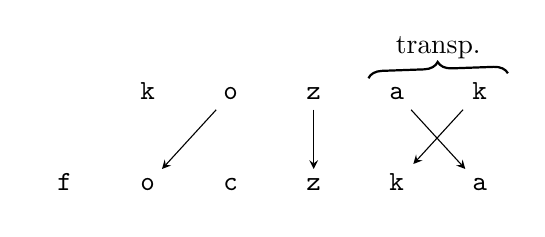
\begin{tikzpicture}
  \matrix (m) [matrix of math nodes,row sep=2em,column sep=1em,minimum width=2em]
  {
  	  & \verb|k| & \verb|o| & \verb|z| & \verb|a| & \verb|k|  \\
  	 \verb|f| & \verb|o| & \verb|c| & \verb|z| & \verb|k| & \verb|a| \\
     };
  \path[-stealth]
    (m-1-3) edge node [left] {} (m-2-2)
           
    (m-1-4) edge node [left] {} (m-2-4)
    
    (m-1-5) edge node [left] {} (m-2-6)
    
    (m-1-6) edge node [left] {} (m-2-5)
    
    ;
      \draw[decorate,decoration={brace,amplitude=5pt},transform canvas={},thick] (m-1-5.north west) -- node[yshift=1em] { transp. } (m-1-6.north east);
      ;

\end{tikzpicture}
\cprotect\caption{Przykład odległości Jaro między napisami \verb|kozak| i \verb|foczka|.}\label{rys:005}
\end{figure}

\begin{example}
Odległość Jaro między napisami \verb|kozak| i \verb|foczka| wynosi: $d_{jaro}(\verb|kozak|, \verb|foczka|)  \approx 0.261$, bo liczba wspólnych znaków wynosi $m = 4$, a liczba potrzebnych transpozycji wynosi $T = 1$ (p. rys.~\ref{rys:005}), co daje odległość równą $d_{jaro}(\verb|kozak|, \verb|foczka|) = 1 - \frac{1}{3}(\frac{3}{5} + \frac{4}{6} + \frac{3}{4}) = \frac{47}{180} \approx 0.261$.
\end{example}

Winkler rozszerzył odległość Jaro poprzez włączenie dodatkowej kary za błędny znak wśród pierwszych czterech znaków napisu~\cite{Loo2014:stringdist}:

\begin{definition}
Niech $s$ i $t$ będą napisami z $\Sigma^*$, $\ell(s,t)$ oznacza długość najdłuższego wspólnego prefiksu, mającego maksymalnie cztery znaki i niech $p$ będzie liczbą z przedziału $[0, \frac{1}{4}]$. Wówczas odległość Jaro-Winklera dana jest wzorem~\cite{Winkler1990:stringcomparator}:

\begin{equation}
\label{eq:012}
d_{jw}(s,t, p) = d_{jaro}(s,t)[1 - p\ell(s,t)]
\end{equation}
\end{definition}

Czynnik $p$ określa jak bardzo różnice w czterech pierwszych znakach w obu napisach wpływają na odległość między nimi. Zmienna $p$ jest liczbą z przedziału $[0, \frac{1}{4}]$, by mieć pewność, że odległość Jaro-Winklera miała wartości w przedziale $[0,1]$ ($0 \leq d_{jw}(s,t) \leq 1$). Jeśli $p=0$, to odległość ta redukuje się do odległości Jaro i wszystkie znaki wnoszą taki sam wkład do funkcji odległości. Jeśli $p = \frac{1}{4}$, to odległość Jaro-Winklera jest równa zero nawet wówczas gdy tylko cztery pierwsze znaki w obu napisach pokrywają się[W LOO JEST BLAD!!]. Powód jest taki, że podobno [PISAC PODOBNO???] ludzie są mniej skłonni do popełniania błędów w czterech pierwszych znakach lub też są one lepiej zauważalne, więc różnice w pierwszych czterech znakach wskazują na większe prawdopodobieństwo, że dwa napisy są rzeczywiście różne~\cite{Loo2014:stringdist}. Wikler~\cite{Winkler1990:stringcomparator} używał w swoich badaniach $p = 0.1$ i zauważył lepsze rezultaty niż dla $p = 0$.

\begin{example}
Odległość Jaro-Winklera między napisami \verb|faktura| i \verb|faktyczny| dla $p = 0$, $p = 0.1$ oraz $p = 0.25$ wynosi odpowiednio: 
\begin{equation*}
  \left.\begin{array}{l@{}l}
    d_{jw}(\verb|faktura|, \verb|faktyczny|, p = 0.00) & \approx 0.328 = d_{jaro}(\verb|faktura|, \verb|faktyczny|) \\
    d_{jw}(\verb|faktura|, \verb|faktyczny|, p = 0.10) & \approx 0.197  \\
    d_{jw}(\verb|faktura|, \verb|faktyczny|, p = 0.25) & =  0
  \end{array}\right.
\end{equation*}
\end{example}

Łatwo zauważyć z równań \ref{eq:011} i \ref{eq:012}, że odległości Jaro i Jaro-Winklera, dla $p \neq \frac{a}{4}$, są nieujemne,  symetryczne i spełniają warunek identycznościowy [DOWOD??]. Nierówność trójkatą w obu przypadkach nie jest jednak spełniona. Rozważmy następujący przykład: $s = \verb|ab|, t = \verb|cb|, u = \verb|cd|$. Jako że napisy $s$ i $u$ nie mają wspólnych znaków, to odległość Jaro między nimi wynosi $d_{jaro}(s, u) = 0$, podczas gdy $d_{jaro}(s, t) = d_{jaro}(t, u) = \frac{1}{3}$, więc w tym przypadku $d_{jaro}(s, u)$ jest większe od $d_{jaro}(s, t) + d_{jaro}(t, u)$. Z tego łatwo zauważyć, że odległość Jaro-Winklera nie spełnia nierówności trójkąta  dla tego samego przykładu dla $p \in [0, \frac{1}{4}]$~\cite{Loo2014:stringdist}.

\subsection{Podsumowanie}

W niniejszym rozdziale przedstawiono odległości określone na napisach [czy też przestrzeni ciągów znaków]. Mając do wyboru wachlarz różnych funkcji nasuwa się pytanie której użyć. Ostateczna decyzja zależy od konkretnego przypadku, jednak istnieją pewne ogólne reguły. Wybór pomiędzy odległościami opartymi na operacjach edycyjnych i $q$-gramach z jednej strony, a miarami heurystycznymi z drugiej zależy w dużej mierze od długości napisów -- te ostatnie są dedykowane krótszym napisom takim jak np. dane osobowe. W odróżnieniu od odległości opartych na operacjach edycyjnych i miarach heurystycznych, odległości oparte na $q$-gramach można łatwo policzyć dla bardzo długich tekstów, jako że liczba $q$-gramów możliwych do utworzenia z języka naturalnego (dla niezbyt małego $q$, tj. $q \geq 3$) jest z reguły o wiele mniejsza niż liczba $q$-gramów, którą można otrzymać z całego alfabetu. Wybór pośród odległości opartych na operacjach edycyjnych zależy przede wszystkim od dokładności jaką chce się otrzymać. Przykładowo do wyszukiwania haseł w słowniku, gdzie różnice między dobranymi napisami są niewielkie, odległości pozwalające na więcej operacji edycyjnych (tak jak np. odległość Damerau-Levenshteina) mogą dać lepsze rezultaty. Odległości Jaro i Jaro-Winklera zostały skonstruowane do krótkich, napisanych przez człowieka, napisów, więc ich zakres zastosowania powinien być jasny.


\chapter{Analiza skupień metodą $k$-średnich}

Analiza skupień polega na wyróżnieniu w zbiorze ustalonej liczby rozłącznych skupień obserwacji w jakimś sensie do siebie podobnych, równocześnie zachowując maksymalne zróżnicowanie obserwacji pomiędzy poszczególnymi podzbiorami~\cite{Koronacki2005:statystyczne}. W niniejszym rozdziale przedstawimy analizę skupień metodą $k$-średnich w trzech odsłonach: przedstawimy metodę wsadową, przy użyciu stochastycznego spadku gradientu oraz metodę pośrednią, tzw. mini-wsadową.

\section{Metoda $k$-średnich}

Rozważmy przestrzeń euklidesową $\mathbb{R}^p$ i niech będzie dana liczba skupień $k$. Wówczas zadanie znalezienia skupień o wyżej wymienionych własnościach można sprowadzić do dobrze określonego zadania optymalizacji. Weźmy próbę $n$-elementową obserwacji $\mathbf{x}_i,\ i = 1,\ldots,n$ o wartościach w $\mathbb{R}^p$. %Niech $d_{ij} = d(\mathbf{x}_i, \mathbf{x}_j)$ oznacza kwadrat odległości między obserwacjami $\mathbf{x}_i$ i $\mathbf{x}_j$. Wówczas 
Suma kwadratów odległości między obserwacjami próby wynosi~\cite{Koronacki2005:statystyczne}
\begin{equation}
T = \frac{1}{2}\sum\limits_{i}^{n}\sum\limits_{j}^{n} \norm{\mathbf{x}_i - \mathbf{x}_j}_2^2,
\end{equation}
gdzie $\norm{\cdot}_2$ oznacza normę euklidesową. Niech funkcja $C:\{1,\ldots,n\} \rightarrow \{1,\ldots, k\}$ oznacza przydzielenie danej obserwacji danemu skupieniu, tzn. jeśli $C(i) = l$, to oznacza, że $\mathbf{x}_i$ należy do $l$-tego skupienia. Zakładając, że dokonano podziału próby na $k$ podzbiorów, można całkowitą sumę kwadratów rozłożyć na sumę kwadratów odległości między obserwacjami z tego samego skupienia oraz na sumę kwadratów odległości między obserwacjami z różnych skupień~\cite{Koronacki2005:statystyczne}:
\begin{equation}
T = W + B = \frac{1}{2}\sum\limits_{l=1}^{k}\sum\limits_{C(i) = k}\sum\limits_{C(j) = k} \norm{\mathbf{x}_i - \mathbf{x}_j}_2^2 + \frac{1}{2}\sum\limits_{l=1}^{k}\sum\limits_{C(i) = k}\sum\limits_{C(j) \neq k} \norm{\mathbf{x}_i - \mathbf{x}_j}_2^2 
\end{equation}

Mając tak sformułowany rozkład sumy $T$ widzimy, że zmieniając podział punktów na skupienia zmienia się zarówno suma $W$, jak i $B$. Można więc sformułować problem analizy skupień jako zadanie minimalizacji sumy $W$ lub, równoważnie, maksymalizacji sumy $B$. Maksymalizacja $B$ to po prostu maksymalizacja rozproszenia punktów z różnych podzbiorów, co jest równoznaczne z minimalizacją rozproszenia punktów z tego samego skupienia. Stąd, rozwiązaniem problemu analizy skupień jest dokonanie takiego podziału próby, aby zminimalizować sumę $W$. Ze względu na złożoność obliczeniową, niemożliwe jest bezpośrednie rozwiązanie tego problemu~\cite{Koronacki2005:statystyczne}.

Przez $n_l$ oznaczmy liczność $l$-tego skupienia i niech $\mathbf{m}_l = \frac{1}{n_l} \sum\limits_{C(i) = k} \mathbf{x}_i$ oznacza wektorową średnią obserwacji z $l$-tego skupienia. Łatwo zauważyć, że~\cite{Koronacki2005:statystyczne}
\begin{equation}
\label{eq:013}
W = \frac{1}{2}\sum\limits_{l=1}^{k}\sum\limits_{C(i) = l} n_l \norm{\mathbf{x}_i - \mathbf{m}_l}_2^2
\end{equation}

Średnie $\mathbf{m}_l$, $l = 1,\ldots, k$ nazywamy \emph{środkami skupień}. Równanie~\ref{eq:013} można uprościć do następującej postaci, która w praktyce jest łatwa w optymalizacji:
\begin{equation}
\label{eq:014}
\widetilde{W} = \frac{1}{2}\sum\limits_{l=1}^{k}\sum\limits_{C(i) = l} \norm{\mathbf{x}_i - \mathbf{m}_l}_2^2 = \frac{1}{2}\sum\limits_{i=1}^{n} \norm{\mathbf{x}_i - \mathbf{m}_{C(i)}}_2^2 
\end{equation}

Algorytmy, które rozwiązują problem minimalizacji sumy~\ref{eq:014}, znane są pod nazwą \emph{metody $k$-średnich}.

\section{Algorytmy}

\subsection{Algorytm wsadowy}


Algorytm \emph{wsadowy} (ang. \emph{batch algorithm}) zostaje zainicjalizowany przez losowe wyznaczenie $k$ punktów jako początkowe środki skupień. Dalej następuje przydzielenie wszystkich punktów próby do najbliższego skupienia, a następnie przeliczenie środków jako średniej ze wszystkich obserwacji w danym skupieniu. Procedura ta jest powtarzana aż do ustabilizowania się algorytmu, tj. do momentu aż żaden punkt próby nie zmieni skupienia~\cite{Wu2007:topten}.

\begin{algorithm}[!h]
\begin{algorithmic}[1]
		\State given: $k$, data set $X$
        \State initialize randomly $m_l, \ \forall l=1, ..., k$
        \Repeat
            \For {$i = 1, \ldots, n$}
                \State $C(i) = \arg \min\limits_{l} \norm{\mathbf{x}_i - \mathbf{m}_l }_2^2 $
            \EndFor
            \For {$l = 1, \ldots, k$}
                \State $\mathbf{m}_l = \frac{1}{n_l}\sum\limits_{C(i) = l} \mathbf{x}_i$
            \EndFor

        \Until{convergence}
\end{algorithmic}
\caption{Algorytm wsadowy $k$-średnich}\label{alg:001}
\end{algorithm}

Algorytm wsadowy jest najbardziej popularnym i najczęściej stosowanym algorytmem, gdyż jest szybki i zazwyczaj daje dobre rezultaty. Jednakowoż jeśli liczba obserwacji w zbiorze jest bardzo duża, to obliczanie średnich z obserwacji we wszystkich skupieniach jest bardzo kosztowne obliczeniowo, zbiegając w czasie $O(knp)$, gdzie $p$ to liczba zmiennych. Stąd Bottou i Bengio~\cite{Bottou1995:convergenceproperties} zaproponowali algorytm oparty na stochastycznym spadku gradientu.

\subsection{Algorytmy oparte na spadku gradientu}

Algorytmy oparte na spadku gradientu są często stosowane np. w regresji liniowej~\cite{Bottou2012:sgdtricks}. Idea polega na szukaniu minimum z danej funkcji kosztu, w kolejnych krokach algorytmu aktualizując zmienną, w kierunku, w którym spadek gradientu był największy. Każda aktualizacja zależy od parametru, zwanego \emph{parametrem uczenia}, który musi być odpowiednio dobrany. W niniejszej sekcji [podrozdziale?] opiszemy trzy algorytmy oparte na spadku gradientu.

%[NIE WIEM CZY PISAĆ TU WIĘCEJ O GRADIENT DESCENT, Z KTOREGO TO WSZYSTKO POCHODZI, CZY SOBIE DAROWAC]

Mając daną funkcję kosztu $\widetilde{W} = \widetilde{W}(\mathbf{m}, \mathbf{x}_i) = \frac{1}{2}\sum\limits_{i=1}^{n} \norm{\mathbf{x}_i - \mathbf{m}_{C(i)}}_2^2 $, możemy znaleźć minimum używając tzw. \emph{spadku gradientu}. W każdej iteracji algorytmu uaktualniamy wektor $\mathbf{m}$ na podstawie gradientu $\widetilde{W}(\mathbf{m}, \mathbf{x}_i)$:
\begin{equation}
\mathbf{m}^{(t+1)}_l = \mathbf{m}_l^{(t)} + \gamma \sum\limits_{i=1}^{n} \frac{\partial \widetilde{W}(\mathbf{m}, \mathbf{x}_i)}{\partial \mathbf{m}}
\end{equation}
gdzie $\gamma$ jest odpowiednio dobranym \emph{parametrem uczenia}[, a $t$ oznacza iterację algorytmu - PISAC TO??]~\cite{Bottou2012:sgdtricks}. Parametrem uczenia, które daje najlepsze rezultaty dla algorytmu $k$-średnich jest $\frac{1}{n_{C(i)}}$. Stąd też algorytm \emph{wsadowego spadku gradientu}, w każdej iteracji algorytmu aktualizuje wektor $\mathbf{m}$ następująco~\cite{Bottou1995:convergenceproperties}:

%Jeśli początkowa wartość zmiennej $\mathbf{m}^(0)$ jest dostatecznie blisko optimum i parametr $\gamma$ jest dobrze dobrany, to algorytm osiąga złożoność liniową.


%licząc pochodną po zmiennej $\mathbf{m}$ [/ gradient z $\mathbf{m}$]: %szukamy minimum, licząc pochodną po $\mathbf{m}$ i przyrównując ją do zera:
\begin{equation}
\mathbf{m}_l^{(t+1)} = \mathbf{m}_l^{(t)} + \sum\limits_{C(i) = l}   \frac{1}{n_l}(\mathbf{x}_i - \mathbf{m}^{(t)}_l) % \sum\limits_{i=1}^{n}\left\{
%\begin{array}{l l}     
 %   \frac{1}{n_l}(\mathbf{x}_i - \mathbf{m}^{(t)}_l), & \text{gdy } l = C(i) \\
  %  0, & \text{wpp.}
%\end{array}\right.
\end{equation}

Algorytm \emph{stochastycznego spadku gradientu}, ozn. SGD, jest daleko idącym uproszczeniem. Zamiast liczyć gradient z $\widetilde{W}(\mathbf{m}, \mathbf{x}_i)$ wprost, każda iteracja estymuje gradient na podstawie \emph{jednej losowo wybranej} obserwacji $\mathbf{x}_i$~\cite{Bottou2012:sgdtricks}:
\begin{equation}
\mathbf{m}_l^{(t+1)} = \mathbf{m}_l^{(t)} + \gamma \frac{\partial \widetilde{W}(\mathbf{m}, \mathbf{x}_i)}{\partial \mathbf{m}}
\end{equation}
gdzie $\gamma$ jest odpowiednio dobranym parametrem uczenia. Tak samo jak w przypadku algorytmu wsadowego, parametrem uczenia, które daje najlepsze rezultaty jest $\frac{1}{n_{C(i)}}$. Stąd też algorytm stochastycznego spadku gradientu w każdej iteracji algorytmu aktualizuje wektor $\mathbf{m}$ następująco~\cite{Bottou1995:convergenceproperties}:

\begin{align}
n^{(t+1)}_l& = n^{(t)}_l + \left\{
\begin{array}{l l}     
    1, & \text{gdy } l = C(j) \\
    0, & \text{wpp.}
\end{array}\right. \\
\mathbf{m}_l^{(t+1)}& = \mathbf{m}_l^{(t)} + \left\{
\begin{array}{l l}     
    \frac{1}{n_l}(\mathbf{x}_i - \mathbf{m}^{(t)}_l), & \text{gdy } l = C(i) \\
    0, & \text{wpp.}
\end{array}\right.
\end{align}


Algorytm SGD opiera się na przeliczaniu średniej po każdym przydzieleniu obserwacji do skupienia, choć z powodu stochastycznego szumu, takie rozwiązanie może nie prowadzić do lokalnego minimum, a jedynie w jego ,,pobliże''. Na rys.~\ref{rys:006} przedstawiono przykładową drogę aktualizacji parametrów. Kolejne elipsy oznaczają stałą wartość funkcji kosztu $\widetilde{W}(\mathbf{m}, \mathbf{x}_i)$ w zależności od wartości zmiennej $\mathbf{m}$, a centrum (środek?) oznacza (lokalne) minimum tej funkcji. Jeśli algorytm rozpoczyna działanie w punkcie oznaczonym przez $X$, to w przypadku algorytmu wsadowego spadku gradientu, w kolejnych iteracjach zmienna $\mathbf{m}$ zmienia swoją wartość, przybliżając się do (lokalnego) minimum funkcji $\widetilde{W}$. Natomiast algorytm stochastycznego spadku gradientu w każdej iteracji przybliża się w stronę minimum w sposób losowy, tzn. może nigdy nie osiągnąć właściwego minimum, a jedynie ,,krążyć'' wokół niego.
 

\begin{figure}[!h]
\centering
\resizebox{8cm}{8cm}{
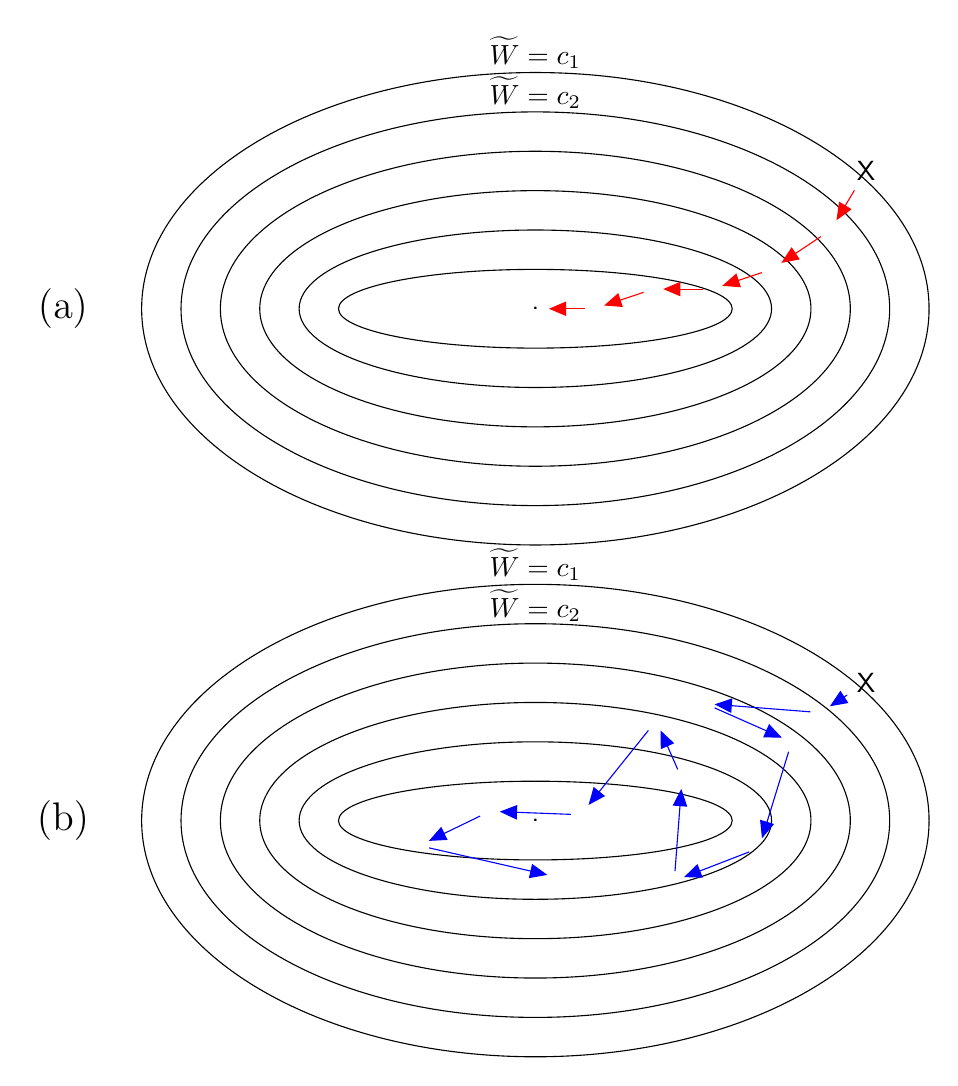
\begin{tikzpicture}[>=triangle 45,font=\sffamily]
    
    \draw (0,6.5) ellipse (5cm and 3cm);
    \draw (0,6.5) ellipse (4.5cm and 2.5cm);
    \draw (0,6.5) ellipse (4cm and 2cm);
    \draw (0,6.5) ellipse (3.5cm and 1.5cm);
    \draw (0,6.5) ellipse (3cm and 1cm);
    \draw (0,6.5) ellipse (2.5cm and 0.5cm);
    \node (B) at (4.2, 8.25) {X};
    \node (C) at (3.75, 7.5) {};
    \node (D) at (3, 7) {};
    \node (E) at (2.25, 6.75) {};
    \node (F) at (1.5, 6.75) {};
    \node (G) at (0.75, 6.5) {};
    \node (H) at (0, 6.5) {.};
    \draw [->, red]  (B) edge (C) (C) edge (D) 
    (D) edge (E) (E) edge (F) (F) edge (G) (G) edge (H);
    \node (c1) at (0, 9.75) {$\widetilde{W} = c_1$};
    \node (c2) at (0, 9.24) {$\widetilde{W} = c_2$};
    
    \draw (0,0) ellipse (5cm and 3cm);
    \draw (0,0) ellipse (4.5cm and 2.5cm);
    \draw (0,0) ellipse (4cm and 2cm);
    \draw (0,0) ellipse (3.5cm and 1.5cm);
    \draw (0,0) ellipse (3cm and 1cm);
    \draw (0,0) ellipse (2.5cm and 0.5cm);
    
	\node (a) at (0, 0) {.};
    \node (b) at (4.2, 1.75) {X};
    \node (c) at (3.617, 1.371) {};
    \node (d) at (2.152, 1.486) {};
    \node (e) at (3.255, 0.998) {};
    \node (f) at (2.840, -0.350) {};
    \node (g) at (1.764, -0.766) {};
    \node (h) at (1.863, 0.526) {};
    \node (i) at (1.535, 1.269) {};
    \node (j) at (0.576, 0.074) {};
    \node (k) at (-0.576, 0.118) {};
    \node (l) at (-1.476, -0.318) {};
    \node (m) at (0.276, -0.718) {};
    \node (c3) at (0, 3.25) {$\widetilde{W} = c_1$};
    \node (c4) at (0, 2.73) {$\widetilde{W} = c_2$};
    
    \draw [->, blue]  (b) edge (c) (c) edge (d) 
    (d) edge (e) (e) edge (f) (f) edge (g) (g) edge (h) (h) edge (i) (i) edge (j) (j) edge (k) (k) edge (l) (l) edge (m);
    
	\node [font=\fontsize{52}{58}] (1) at (-6, 6.5) {\Large(a)};
    \node [font=\fontsize{52}{58}] (2) at (-6, 0) {\Large(b)};
        
\end{tikzpicture}
}
\caption{Przykładowa droga wsadowego spadku gradientu (rys. a) i stochastycznego spadku gradientu (rys. b).}\label{rys:006}
\end{figure}



Algorytm oparty na stochastycznym spadku gradientu (znany również pod nazwą algorytmu \emph{online'owego} [I TAK I NIE - ZALEZY OD ARTICLE'A]) rozpoczyna się tak samo, tj. inicjalizacją losowych $k$ środków skupień. Następnie zbiór obserwacji jest mieszany i obserwacje po kolei są przydzielane do najbliższego skupienia. Środki skupień przeliczane są po każdym przydzieleniu punktu do skupienia. Procedura ta powtarzana jest $t$ razy~\cite{Bottou1995:convergenceproperties}. Algorytm ten jest dużo szybszy od dwóch wcześniejszych, kosztem dokładności rozwiązania~\cite{Bottou2012:sgdtricks}.

\begin{algorithm}[h!]
\begin{algorithmic}[1]
		\State given: $k$, data set $X$, iterations $t$
        \State initialize randomly $m_l, \ \forall l=1, ..., k$
        \State initialize $n_l = 0, \ \forall l=1, ..., k$
        \For {$a = 1, \ldots, t $}
        	\State randomly pick one observation $\mathbf{x}_i$ from $X$
            %\For {$i = 1, \ldots, n$}
                \State $C(i) = \arg \min\limits_{l} \norm{\mathbf{x}_i - \mathbf{m}_l }_2^2 $
                \State $n_{C(i)} = n_{C(i)} + 1$
                \State $\mathbf{m}_{C(i)} = \mathbf{m}_{C(i)} + \frac{1}{n_{C(i)}}\norm{\mathbf{x}_i - \mathbf{m}_{C(i)}}_2$
            %\EndFor
       \EndFor
\end{algorithmic}
\caption{Algorytm SGD $k$-średnich}\label{alg:002}
\end{algorithm}

Algorytm \emph{mini-wsadowy} (ang. \emph{mini-batch $k$-means}) jest połączeniem dwóch poprzednich algorytmów, tj. w każdej iteracji przydzielanych do najbliższego skupienia jest $b$ losowo wybranych obserwacji, po czym następuje przeliczenie środków skupień~\cite{Sculley2010:webkmeans}. Algorytm ten jest porównywalnie szybki do algorytmu SGD, osiągając przy tym lepsze rezultaty z powodu mniejszego stochastycznego szumu.

\begin{algorithm}[h!]
\begin{algorithmic}[1]
		\State given: $k$, data set $X$, iterations $t$, mini-batch size $b$
        \State initialize randomly $m_l, \ \forall l=1, ..., k$
        \State initialize $n_l = 0, \ \forall l=1, ..., k$
        \For {$a = 1, \ldots, t $}
        	%\State shuffle data set $X$
        	\State $B = b$ observations randomly picked from $X$
            \For {$i : \mathbf{x}_i \in B$}
                \State $C(i) = \arg \min\limits_{l} \norm{\mathbf{x}_i - \mathbf{m}_l }_2^2 $
            \EndFor
            \For {$i : \mathbf{x}_i \in B$}
                \State $n_{C(i)} = n_{C(i)} + 1$
                \State $\mathbf{m}_{C(i)} = \mathbf{m}_{C(i)} + \frac{1}{n_{C(i)}}\norm{\mathbf{x}_i - \mathbf{m}_{C(i)}}_2$
            \EndFor
       \EndFor
\end{algorithmic}
\caption{Algorytm mini-wsadowy $k$-średnich}\label{alg:003}
\end{algorithm}

[CZY PODAWAC TUTAJ PRZYKLAD + RYSUNKI Z \cite{Sculley2010:webkmeans} O TYM ZE MINI-BATCH JEST TAKI SUPER W POR. Z INNYMI??]


\section{Metody oceny klasyfikacji}


%-----------Koniec części zasadniczej-----------


\bibliographystyle{plain}
\bibliography{bibliography}

%\makestatement
\end{document}
